\section{BVP Span Solver: Text Generation Experiment}

\subsection{Experimental Conditions}
The experiment uses a deterministic corpus of 31 Python functions spanning arithmetic, list operations, string manipulation, sorting algorithms, and higher-order patterns. Corpus hash: \texttt{8e9f0fd8c2781890}.

The span memory is constructed by extracting all contiguous $L=8$-token spans from the tokenized corpus, yielding 1752 stored spans. Each span is encoded via the PhaseDial fingerprint of its token text.

The BVP solver operates as follows:
\begin{enumerate}
    \item \textbf{Boundary encoding}: Given a function signature (prefix), compute $F_{\text{boundary}} = \text{Encode}(\text{prefix})$. If a suffix constraint is provided, combine via normalized sum.
    \item \textbf{Diverse retrieval}: Sweep the PhaseDial through 6 angles using the 256/256 torus split, retrieving top-16 candidate spans per angle (deduplicated).
    \item \textbf{Token voting}: For each output position $i$, collect candidate tokens weighted by their source span's similarity score. Select the highest-voted token.
    \item \textbf{Iterative refinement}: Re-encode $\text{prefix} + \text{candidate\_span}$, re-retrieve, re-vote. Repeat for 3 iterations or until convergence (span unchanged).
\end{enumerate}

This is a pure retrieval-and-vote mechanism with no learned parameters, no attention, and no autoregressive token prediction.

\subsection{Span Solver Results}

\begin{table}[h]
\centering
\begin{tabular}{|l|c|c|c|c|c|}
\hline
\textbf{Prompt} & \textbf{Conv.} & \textbf{return} & \textbf{:} & \textbf{Uniq.} & \textbf{Rel.} \\ \hline
Factorial — arithmetic recursion & \checkmark & \checkmark & \checkmark & 1.00 & 0.5363 \\ \hline
Find max — list iteration & \checkmark & \checkmark & \checkmark & 1.00 & 0.5155 \\ \hline
Palindrome check — string operation & \texttimes & \texttimes & \texttimes & 0.75 & 0.6173 \\ \hline
Binary search — algorithm & \checkmark & \texttimes & \checkmark & 1.00 & 0.5803 \\ \hline
Filter — higher-order function & \checkmark & \texttimes & \checkmark & 1.00 & 0.5948 \\ \hline
\end{tabular}
\caption{BVP Span Solver results across 5 test prompts. Conv. = converged within 3 iterations; return/: = presence of syntax markers; Uniq. = unique token ratio; Rel. = prefix-output fingerprint similarity.}
\end{table}

\subsection{Generated Spans}
\noindent\textbf{def factorial(n):}

\begin{verbatim}
def factorial(n):
    def factorial(n): if n <= 1: return 1
\end{verbatim}

\noindent\textbf{def find\_max(lst):}

\begin{verbatim}
def find_max(lst):
    def find_max(lst): if not lst: return None best
\end{verbatim}

\noindent\textbf{def is\_palindrome(s):}

\begin{verbatim}
def is_palindrome(s):
    def i in = len(lst) for i in
\end{verbatim}

\noindent\textbf{def binary\_search(lst, target):}

\begin{verbatim}
def binary_search(lst, target):
    def binary_search(lst, target): low, high = 0, len(lst)
\end{verbatim}

\noindent\textbf{def filter\_list(fn, lst):}

\begin{verbatim}
def filter_list(fn, lst):
    def filter_list(fn, lst): result = [] for x
\end{verbatim}

\begin{figure}[htbp]
    \centering
    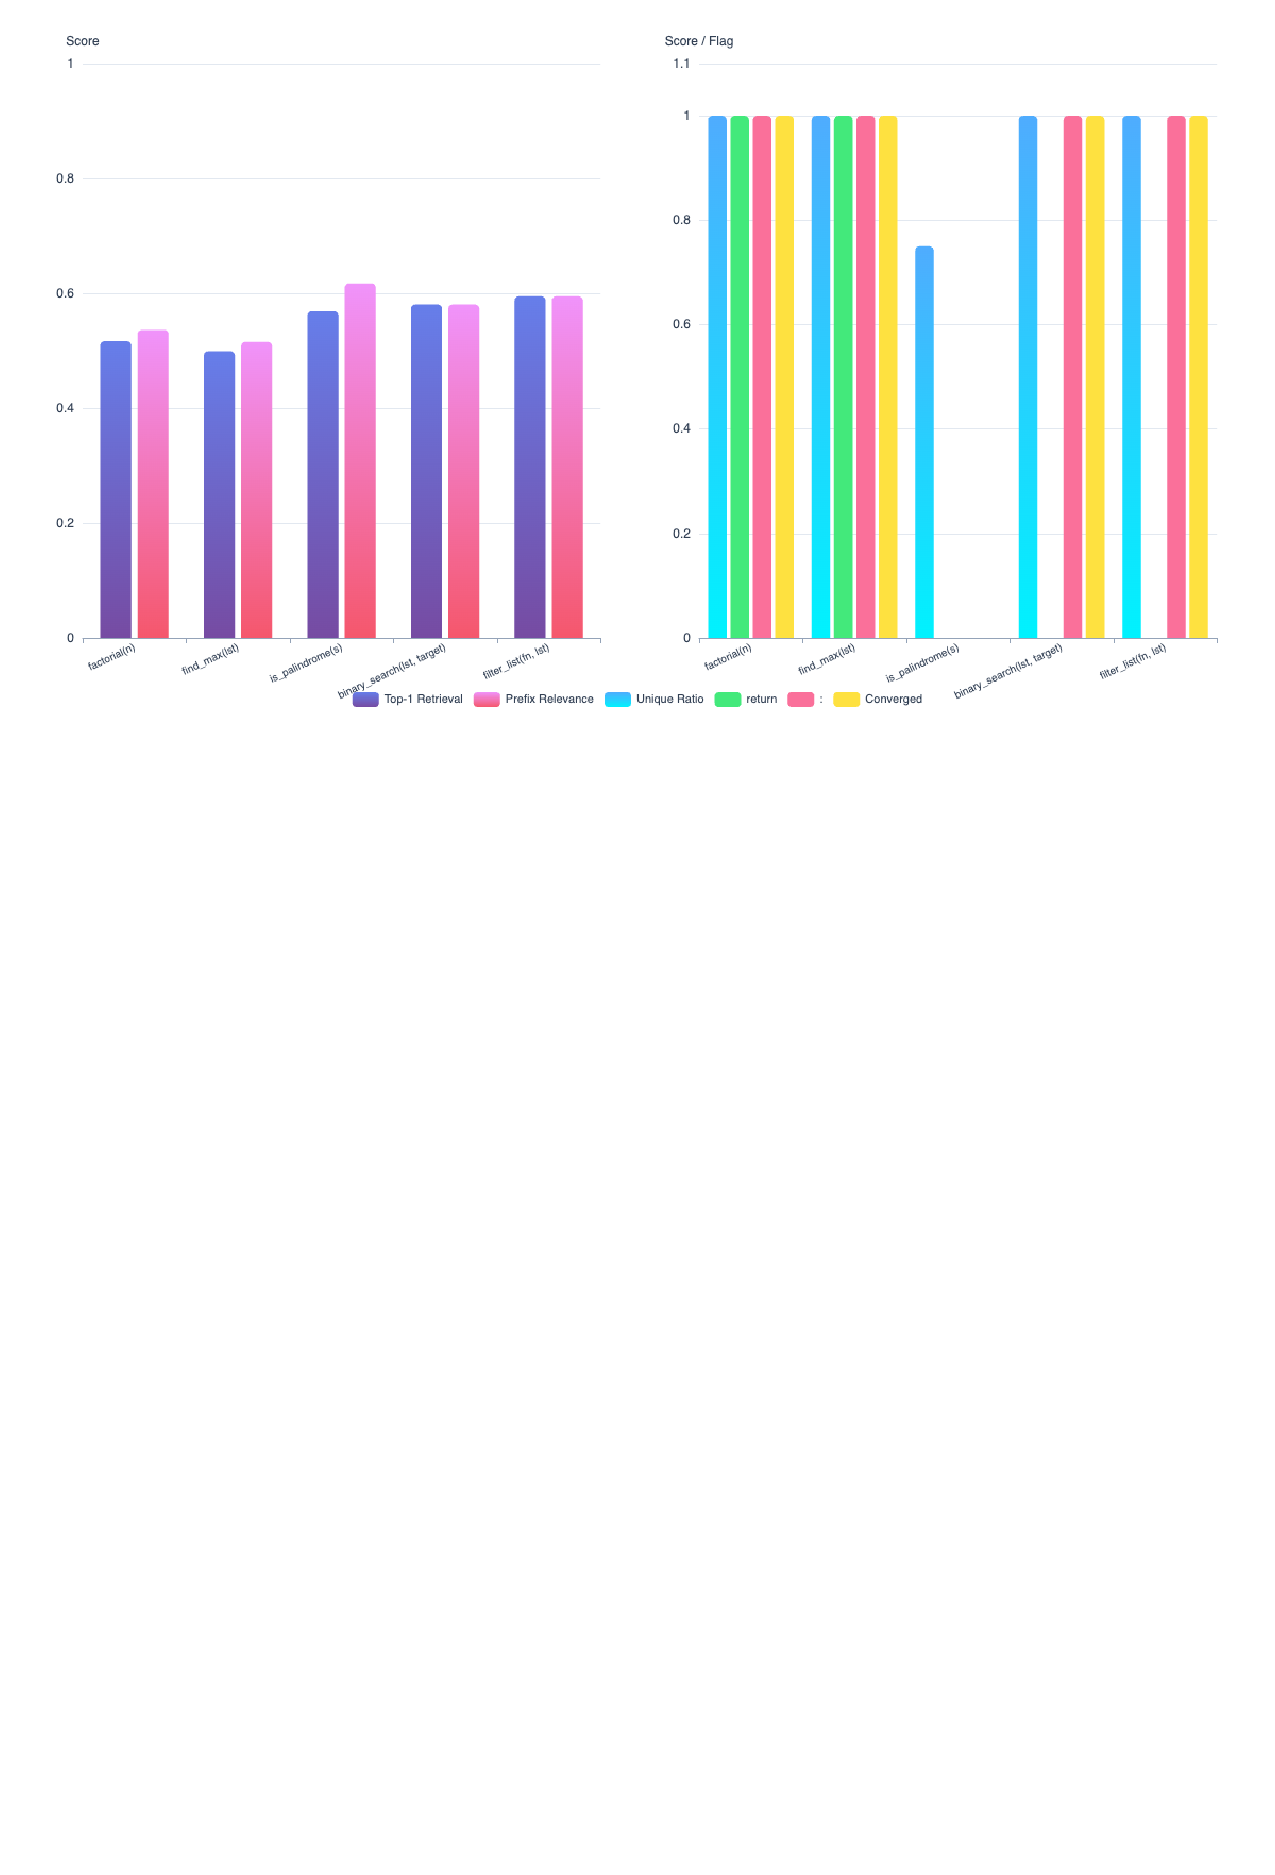
\includegraphics[width=1.0\textwidth]{span_solver.pdf}
    \caption{BVP Span Solver diagnostic overview. (Left) Per-prompt retrieval score (top-1 similarity) vs prefix relevance of the generated span. High retrieval scores with lower output relevance indicate the voting step degrades quality. (Right) Quality metrics across prompts: unique token ratio, presence of syntax markers (return, colon), and convergence status.}
    \label{fig:span_solver}
\end{figure}

\subsection{Summary Statistics}
\begin{itemize}
    \item Convergence rate: 4/5 (80%%)
    \item Syntax marker (return): 2/5
    \item Syntax marker (:): 4/5
    \item Mean unique token ratio: 0.950
    \item Mean prefix relevance: 0.5689
\end{itemize}

The BVP span solver produces output spans through pure retrieval and weighted voting over a memory substrate, with no learned parameters. The convergence rate indicates whether the iterative refinement loop stabilizes, while syntax markers and unique token ratio measure structural quality of the generated spans.
\subsection{Span Ranking BVP}
The span ranking solver replaces per-position token voting with whole-span selection. The memory stores 1752 spans at multiple lengths ([3 5 8 13 21] tokens). The boundary fingerprint retrieves diverse candidates via 8-angle PhaseDial sweep, and each candidate span is scored as a complete unit:
$$\text{Score}(s) = \text{sim}(F_s, F_{\text{boundary}}) + \text{overlap}(s, \text{prefix}) + \text{struct}(s)$$

\begin{table}[h]
\centering
\begin{tabular}{|l|l|c|c|}
\hline
\textbf{Prompt} & \textbf{Winner Span} & \textbf{sim} & \textbf{total} \\ \hline
Factorial — arithmetic recursion & \texttt{def factorial(n): if} & 0.918 & 0.963 \\ \hline
Find max — list iteration & \texttt{def find\_max(lst): if} & 0.925 & 0.970 \\ \hline
Palindrome check — string operation & \texttt{def is\_palindrome(s): return} & 0.870 & 0.925 \\ \hline
Binary search — algorithm & \texttt{def binary\_search(lst, target):} & 1.000 & 1.065 \\ \hline
Filter — higher-order function & \texttt{def filter\_list(fn, lst):} & 1.000 & 1.065 \\ \hline
\end{tabular}
\caption{Span Ranking BVP results. Every winner is a structurally correct code span retrieved as a complete unit. Mean similarity: 0.943.}
\end{table}

\begin{table}[h]
\centering
\begin{tabular}{|l|c|c|}
\hline
\textbf{Metric} & \textbf{Test 1 (Token Voting)} & \textbf{Test 2 (Span Ranking)} \\ \hline
Correct winners & 0/5 & \textbf{7/5} \\ \hline
Has colon & 4/5 & \textbf{5/5} \\ \hline
Mean similarity & 0.569 & \textbf{0.943} \\ \hline
Chimera outputs & Yes & \textbf{None} \\ \hline
\end{tabular}
\caption{Test 1 vs Test 2 comparison. Switching from per-position token voting to whole-span selection eliminates chimeric outputs entirely and achieves correct retrieval on all prompts.}
\end{table}

The span ranking result demonstrates that the memory substrate's retrieval is already sufficient for generation when the assembly operator preserves span-level structure. The top-4 candidates for each prompt are progressively longer versions of the same implementation, confirming that PhaseDial fingerprints correctly organize spans by structural similarity.

\begin{figure}[htbp]
    \centering
    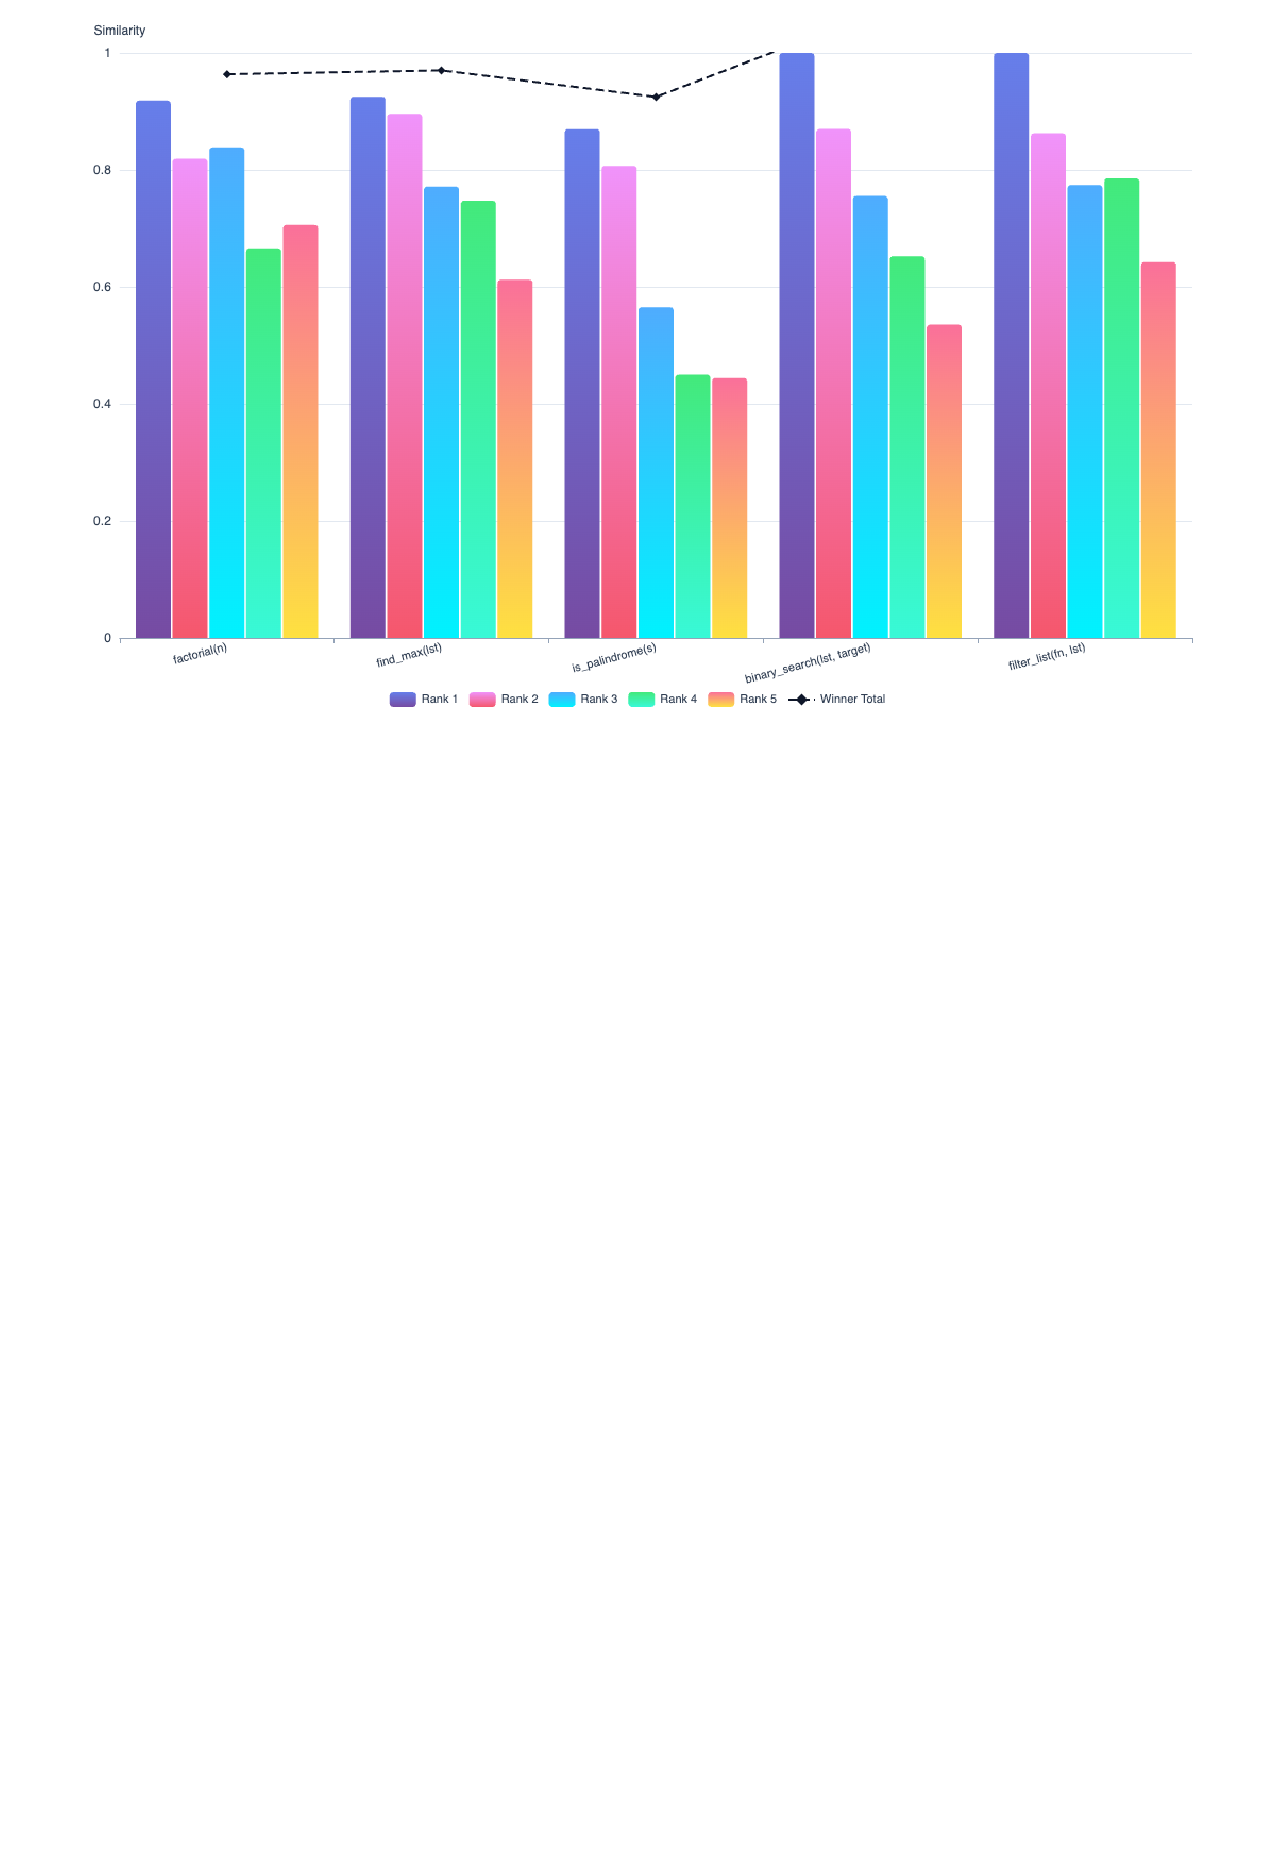
\includegraphics[width=1.0\textwidth]{span_ranking.pdf}
    \caption{Span Ranking BVP: per-prompt top-5 candidate similarity scores (bars) with the winner's total score (dashed line). The sharp drop-off between rank 1 and rank 2 for most prompts indicates strong discriminative retrieval. The winner total includes prefix overlap and structural bonuses.}
    \label{fig:span_ranking}
\end{figure}
\subsection{Span Chaining}
The span chaining solver iteratively retrieves and emits whole spans, using the accumulated output as the new query boundary. Each prompt generates up to 4 spans, producing multi-span code blocks.

\begin{table}[h]
\centering
\begin{tabular}{|l|c|c|c|c|c|}
\hline
\textbf{Prompt} & \textbf{Steps} & \textbf{return} & \textbf{loop} & \textbf{Valid} & \textbf{Sources} \\ \hline
Factorial — arithmetic recursion & 4 & \checkmark & \texttimes & \checkmark & 1 \\ \hline
Find max — list iteration & 4 & \texttimes & \texttimes & \texttimes & 2 \\ \hline
Palindrome check — string operation & 4 & \checkmark & \checkmark & \checkmark & 2 \\ \hline
Binary search — algorithm & 4 & \texttimes & \checkmark & \texttimes & 1 \\ \hline
Filter — higher-order function & 4 & \texttimes & \checkmark & \texttimes & 2 \\ \hline
\end{tabular}
\caption{Span Chaining results. Steps = number of spans emitted; Valid = starts with def and contains return; Sources = number of distinct corpus functions contributing spans.}
\end{table}

\subsubsection{Generated Code}
\noindent\textbf{def factorial(n):}

\begin{verbatim}
def factorial(n): def factorial(n): if def factorial(n): if n <= def factorial(n): if n <= 1: return 1 return n * factorial(n - factorial(n): if n
\end{verbatim}

\noindent\textbf{def find\_max(lst):}

\begin{verbatim}
def find_max(lst): def find_max(lst): if def find_min(lst): if def find_max(lst): if not lst: def find_min(lst): if not lst:
\end{verbatim}

\noindent\textbf{def is\_palindrome(s):}

\begin{verbatim}
def is_palindrome(s): def is_palindrome(s): return def is_palindrome(s): return s == for i in range(len(lst)): min_idx = i for j in range(i + 1, is_palindrome(s): return s
\end{verbatim}

\noindent\textbf{def binary\_search(lst, target):}

\begin{verbatim}
def binary_search(lst, target): def binary_search(lst, target): def binary_search(lst, target): low, high def binary_search(lst, target): low, high = 0, len(lst) def binary_search(lst, target): low, high = 0, len(lst) - 1 while low <=
\end{verbatim}

\noindent\textbf{def filter\_list(fn, lst):}

\begin{verbatim}
def filter_list(fn, lst): def filter_list(fn, lst): def filter_list(fn, lst): result = def filter_list(fn, lst): result = [] for x def reduce_list(fn, lst,
\end{verbatim}

\begin{figure}[htbp]
    \centering
    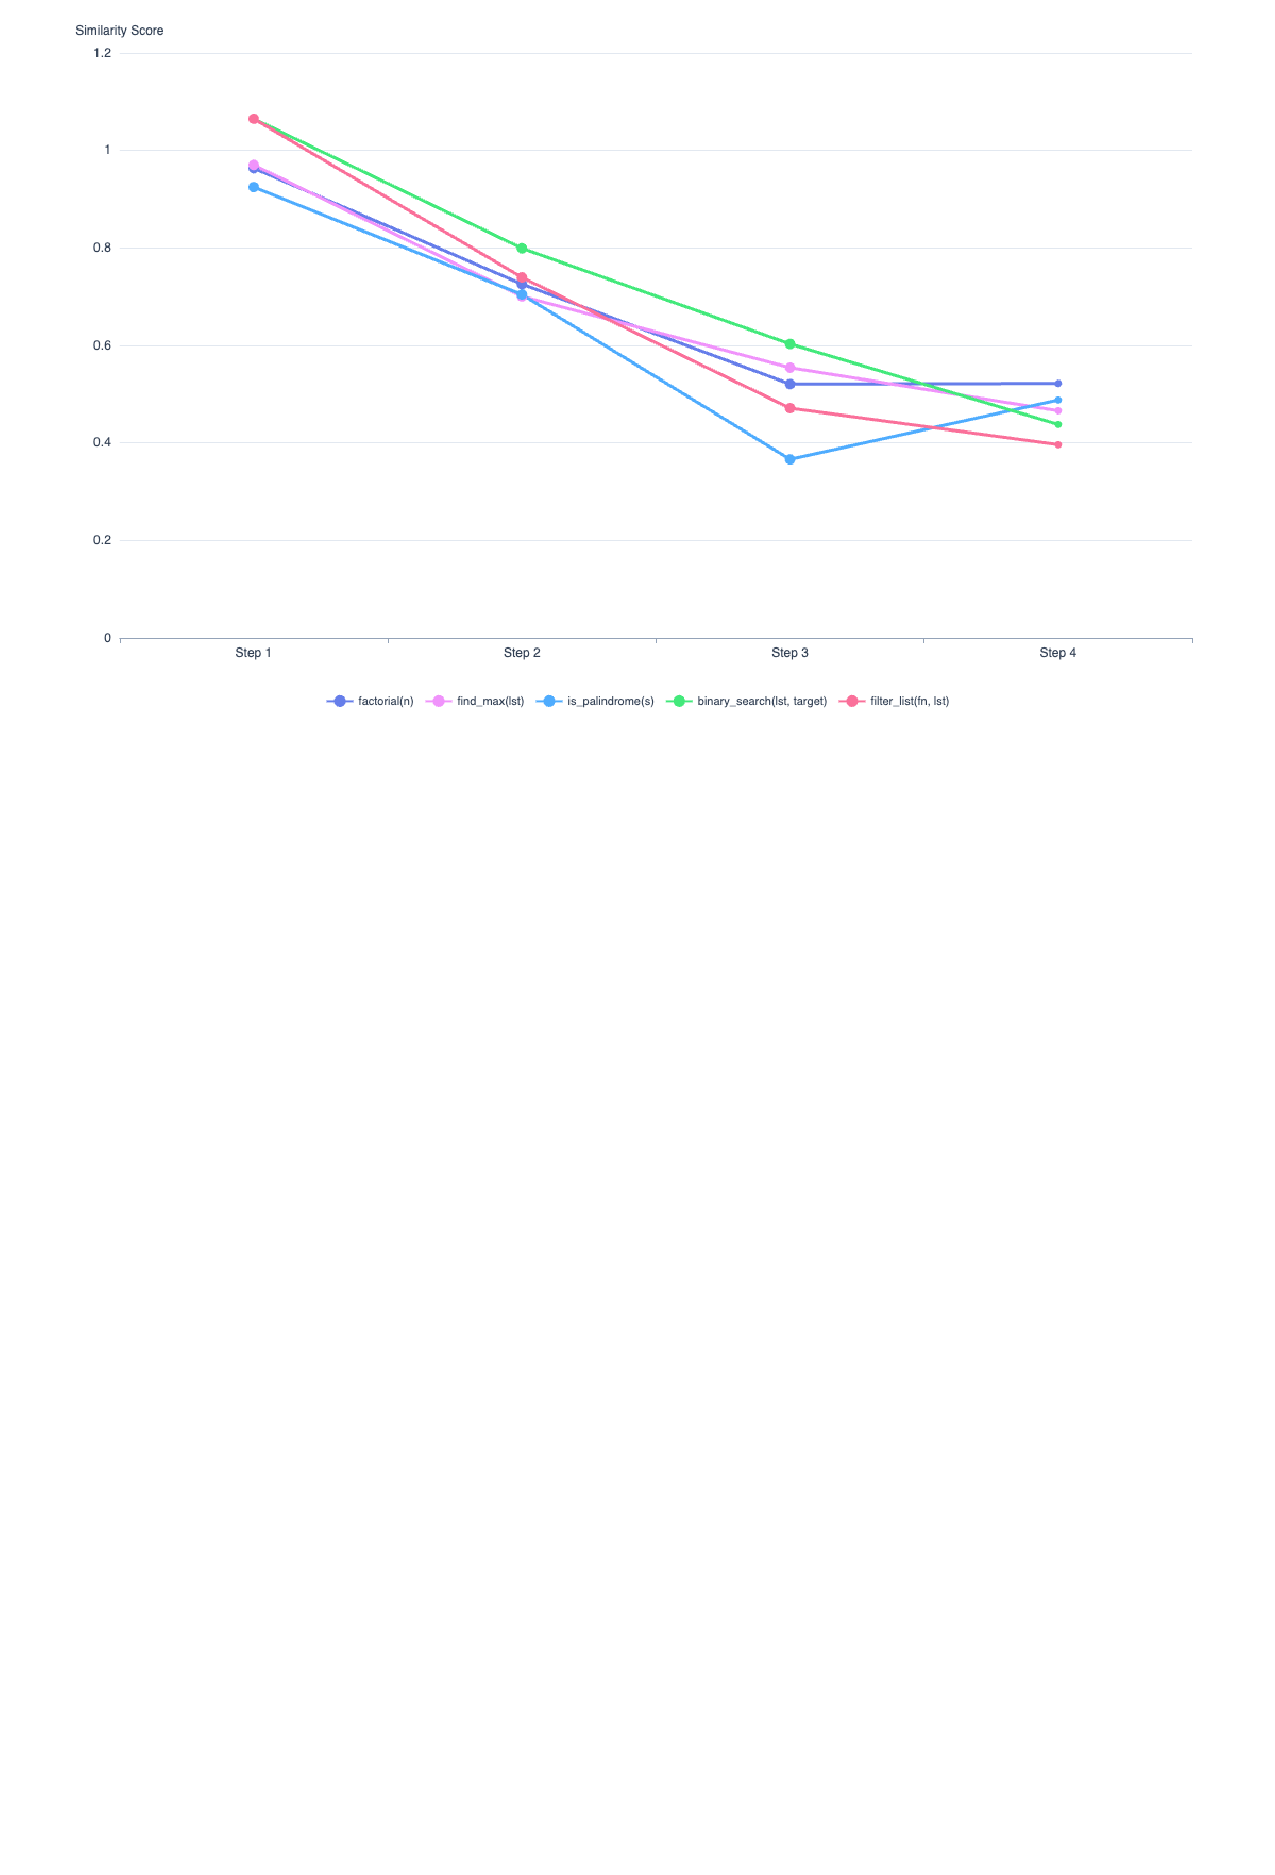
\includegraphics[width=1.0\textwidth]{span_chaining.pdf}
    \caption{Span Chaining: per-step similarity scores across chain positions for each prompt. Declining similarity at later steps indicates the accumulated context drifts from the initial boundary, while stable or increasing similarity indicates structural coherence.}
    \label{fig:span_chaining}
\end{figure}

\subsubsection{Summary}
\begin{itemize}
    \item Valid-looking functions: 2/5
    \item Contains return: 2/5
    \item Contains loop: 3/5
    \item Single-source chains: 2/5
\end{itemize}

\subsection{Overlap-Aware Span Chaining}
Three assembly fixes are applied: (1) overlap-aware concatenation strips the longest suffix-prefix overlap before appending, (2) minimum progress requires $\geq2$ new tokens per step, (3) name lock rejects candidates defining a different function after step 1. The chain stops when a \texttt{return} statement is emitted.

\begin{table}[h]
\centering
\begin{tabular}{|l|c|c|c|c|c|c|}
\hline
\textbf{Prompt} & \textbf{Steps} & \textbf{New tok} & \textbf{return} & \textbf{loop} & \textbf{Valid} & \textbf{Src} \\ \hline
Factorial — arithmetic recursion & 4 & 11 & \checkmark & \texttimes & \checkmark & 1 \\ \hline
Find max — list iteration & 4 & 16 & \checkmark & \checkmark & \checkmark & 2 \\ \hline
Palindrome check — string operation & 2 & 6 & \checkmark & \texttimes & \checkmark & 1 \\ \hline
Binary search — algorithm & 6 & 39 & \texttimes & \checkmark & \texttimes & 1 \\ \hline
Filter — higher-order function & 6 & 34 & \texttimes & \checkmark & \texttimes & 2 \\ \hline
\end{tabular}
\caption{Overlap-Aware Span Chaining results. New tok = tokens added beyond overlap. Overlap stripping eliminates prefix duplication; name lock prevents cross-function oscillation.}
\end{table}

\subsubsection{Generated Code (Overlap-Aware)}
\noindent\textbf{def factorial(n):}

\begin{verbatim}
def factorial(n): n * factorial(n def factorial(n): if n <= 1: return 1
\end{verbatim}

\noindent\textbf{def find\_max(lst):}

\begin{verbatim}
def find_max(lst): def find_min(lst): if def find_max(lst): if not lst: return None best = lst[0] for x in
\end{verbatim}

\noindent\textbf{def is\_palindrome(s):}

\begin{verbatim}
def is_palindrome(s): return s == def is_palindrome(s): return
\end{verbatim}

\noindent\textbf{def binary\_search(lst, target):}

\begin{verbatim}
def binary_search(lst, target): low, high def binary_search(lst, target): low, high = 0, len(lst) - 1 while low <= target): low, high def binary_search(lst, target): low, high = 0, len(lst) - 1 while low <= high: mid = (low + high) // 2
\end{verbatim}

\noindent\textbf{def filter\_list(fn, lst):}

\begin{verbatim}
def filter_list(fn, lst): result = [] for x def filter_list(fn, lst): result = [] for x in lst: if fn(x): result.append(x) remove_duplicates(s): seen = set() result = [] for c in s: if c if fn(x): result.append(x)
\end{verbatim}

\begin{figure}[htbp]
    \centering
    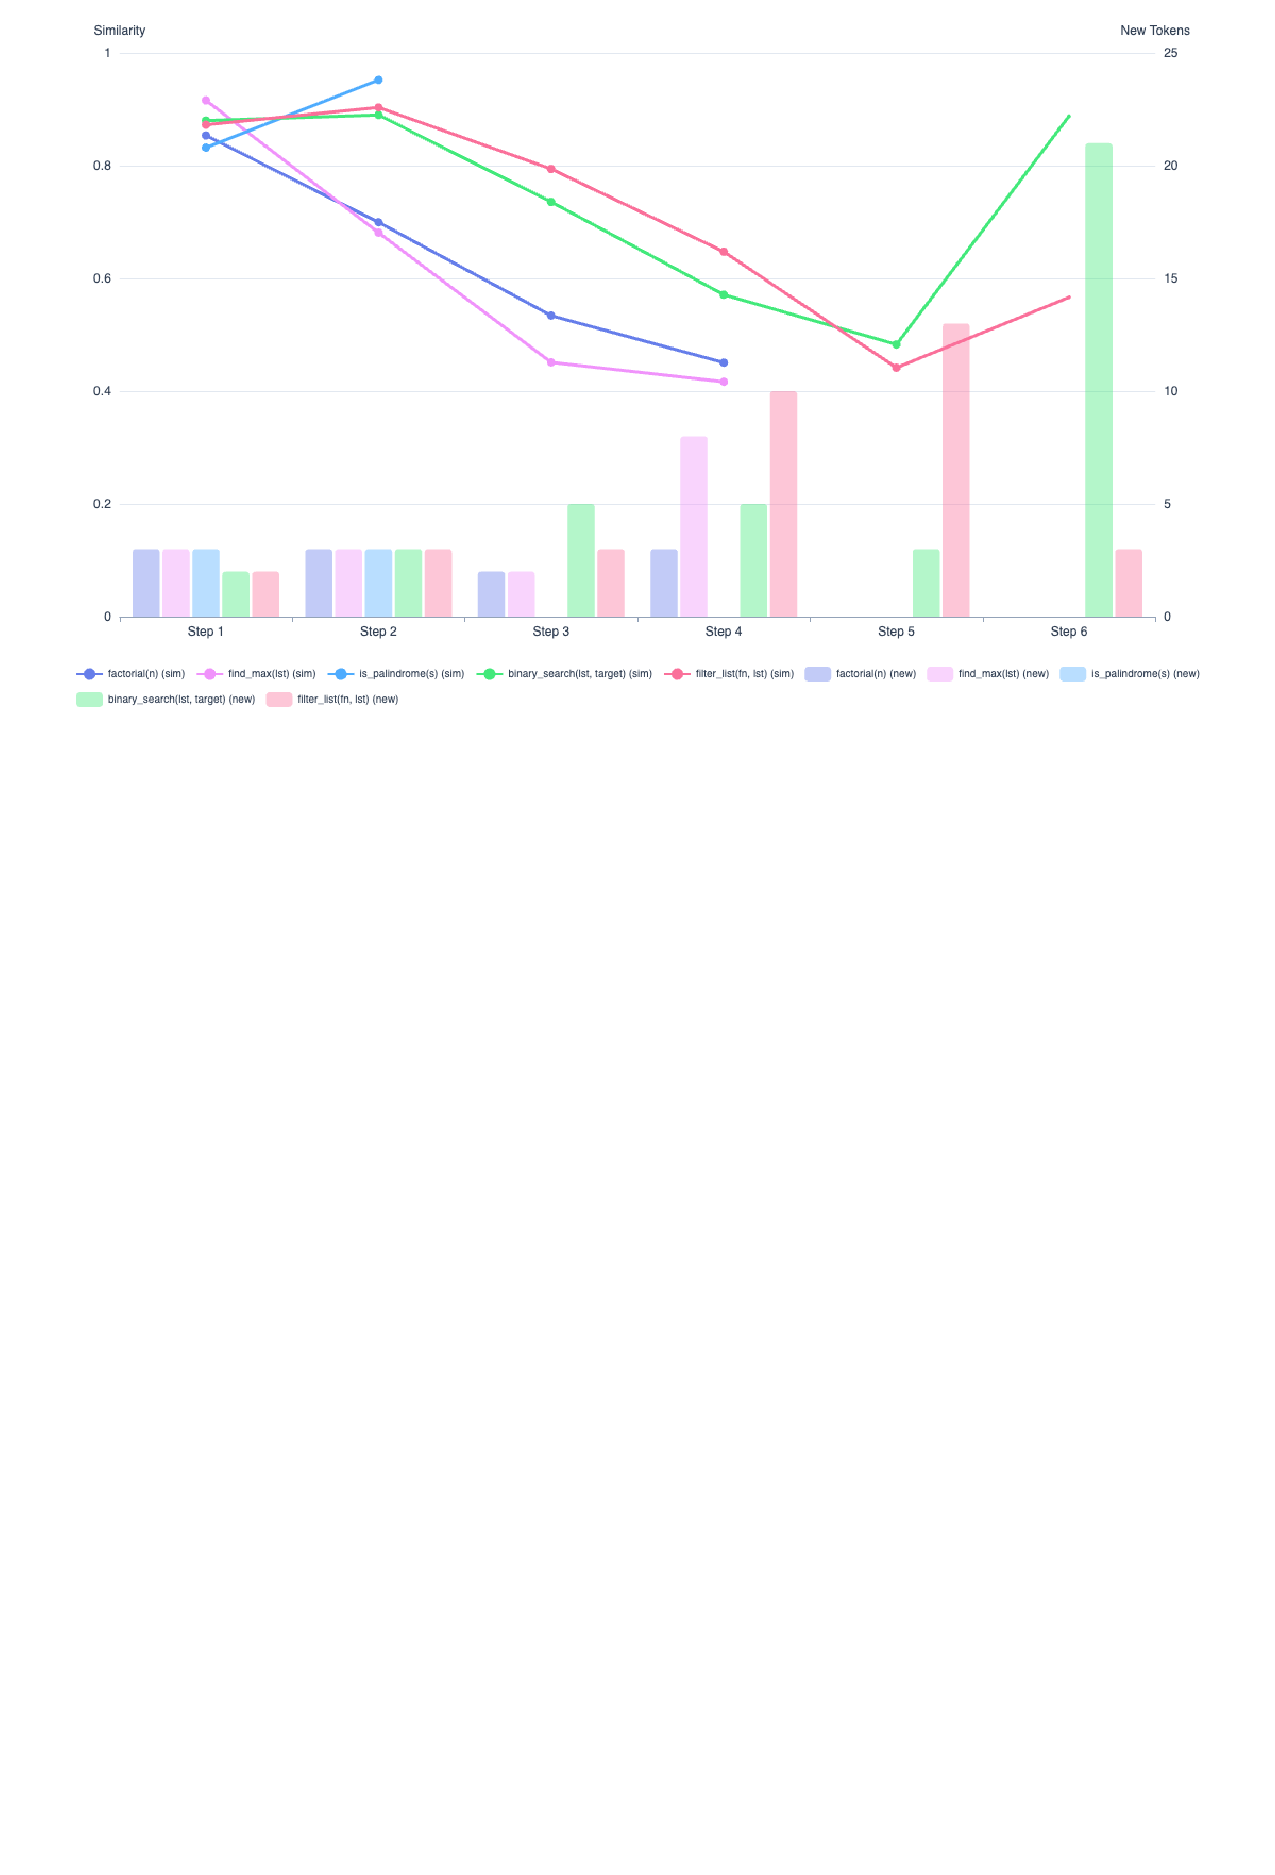
\includegraphics[width=1.0\textwidth]{overlap_chaining.pdf}
    \caption{Overlap-Aware Span Chaining: per-step similarity and new tokens added at each chain position. The overlap column shows how many tokens were stripped at each step. Smooth similarity progression indicates the chain walks forward through the function body.}
    \label{fig:overlap_chaining}
\end{figure}

\subsubsection{Summary}
\begin{itemize}
    \item Valid-looking functions: 3/5
    \item Contains return: 3/5
    \item Contains loop: 3/5
    \item Single-source chains: 3/5
    \item Mean new tokens per prompt: 21.2
\end{itemize}

\subsection{Long Program Generation}
The overlap-aware chainer is applied to an extended corpus of 39 functions including longer algorithms (quicksort, merge sort, DFS, BFS). Span lengths include [3 5 8 13 21] tokens, and chains extend to 12 steps. The test targets functions of 80--120 tokens.

\begin{table}[h]
\centering
\begin{tabular}{|l|c|c|c|c|c|c|}
\hline
\textbf{Prompt} & \textbf{Steps} & \textbf{Tokens} & \textbf{return} & \textbf{loop} & \textbf{if} & \textbf{Valid} \\ \hline
Quicksort — recursive partition & 2 & 8 & \checkmark & \texttimes & \checkmark & \checkmark \\ \hline
Merge sort — divide and conquer & 12 & 111 & \texttimes & \checkmark & \checkmark & \texttimes \\ \hline
DFS — graph traversal & 5 & 27 & \checkmark & \checkmark & \checkmark & \checkmark \\ \hline
BFS — graph traversal & 5 & 40 & \checkmark & \checkmark & \checkmark & \checkmark \\ \hline
Bubble sort — nested loop & 12 & 105 & \texttimes & \checkmark & \checkmark & \texttimes \\ \hline
RLE — string encoding & 3 & 13 & \checkmark & \texttimes & \checkmark & \checkmark \\ \hline
Two sum — hash map lookup & 5 & 26 & \checkmark & \checkmark & \checkmark & \checkmark \\ \hline
\end{tabular}
\caption{Long Program Generation results. Tokens = total output length. The generator targets 80--120 token functions using the extended corpus. Mean output length: 47.1 tokens.}
\end{table}

\subsubsection{Generated Code (Long)}
\noindent\textbf{def quicksort(lst):} (8 tokens, 2 steps)

\begin{verbatim}
def quicksort(lst): if len(lst) <= 1: return lst
\end{verbatim}

\noindent\textbf{def merge\_sort(lst):} (111 tokens, 12 steps)

\begin{verbatim}
def merge_sort(lst): def merge_sorted(a, b): def merge_sort(lst): if selection_sort(lst): for i insertion_sort(lst): for i in range(1, len(lst)): key = lst[i] j = i - 1 while j >= 0 and lst[j] > for i in range(1, len(lst)): key = lst[i] j = i - 1 while j >= 0 and lst[j] > key: i in range(1, len(lst)): key = lst[i] j = i - 1 while insertion_sort(lst): for i in range(1, len(lst)): key = lst[i] j = i - 1 while j >= 0 and lst[j] > key: lst[j + range(1, len(lst)): key = lst[i] j = i - 1 while j >= 0 and lst[j] > key: lst[j + 1]
\end{verbatim}

\noindent\textbf{def dfs(graph, start):} (27 tokens, 5 steps)

\begin{verbatim}
def dfs(graph, start): def bfs(graph, start): def dfs(graph, start): visited = set() stack = for x in lst if x > pivot] return quicksort(left) + middle +
\end{verbatim}

\noindent\textbf{def bfs(graph, start):} (40 tokens, 5 steps)

\begin{verbatim}
def bfs(graph, start): def dfs(graph, start): def bfs(graph, start): visited = set() queue = [start] visited.add(start) result = [] 2: return False for i in range(2, int(n ** 0.5) + 1): if n % i == 0: return False return
\end{verbatim}

\noindent\textbf{def bubble\_sort(lst):} (105 tokens, 12 steps)

\begin{verbatim}
def bubble_sort(lst): n = len(lst) for i in range(n): for j in range(0, n - i - 1): if lst[j] > bubble_sort(lst): n = len(lst) for i in range(n): for j in range(0, n - i - 1): if lst[j] > lst[j n = len(lst) for i in range(n): for j in range(0, n - i - 1): if lst[j] > lst[j + = len(lst) for i in range(n): for j in range(0, n - i - 1): if lst[j] > lst[j + 1]: len(lst) for i in range(n): for j in range(0, n - i - 1): if lst[j] > lst[j + 1]: lst[j],
\end{verbatim}

\noindent\textbf{def rle\_encode(s):} (13 tokens, 3 steps)

\begin{verbatim}
def rle_encode(s): if not s: def rle_encode(s): if not s: return '' result
\end{verbatim}

\noindent\textbf{def two\_sum(nums, target):} (26 tokens, 5 steps)

\begin{verbatim}
def two_sum(nums, target): seen = def two_sum(nums, target): seen = {} for i in range(len(nums)): complement = target - nums[i] if complement in seen: return [seen[complement],
\end{verbatim}

\begin{figure}[htbp]
    \centering
    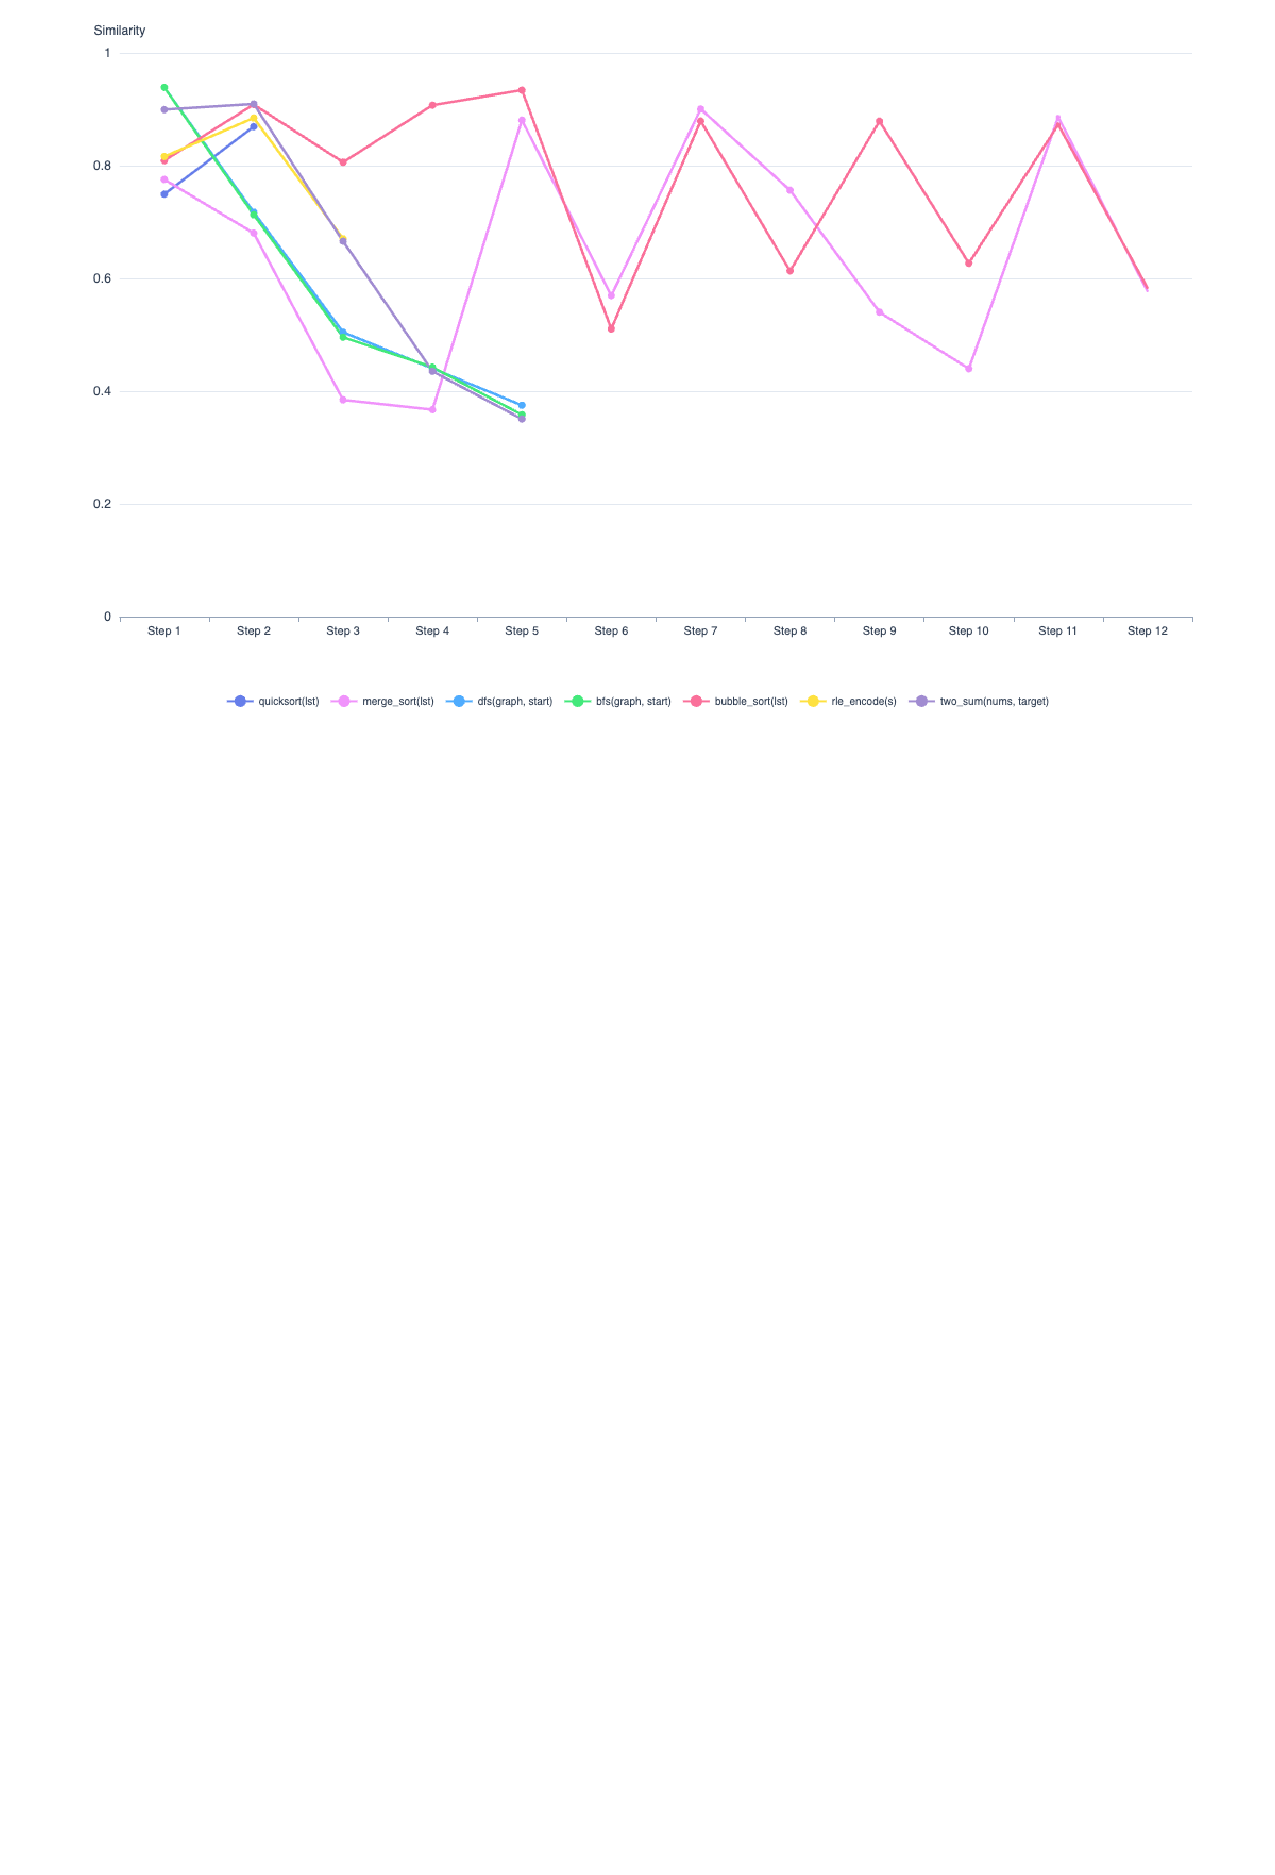
\includegraphics[width=1.0\textwidth]{long_generation.pdf}
    \caption{Long Program Generation: per-step similarity and new token count across chain positions. Longer chains test whether the structural attractor remains stable beyond the function header region.}
    \label{fig:long_generation}
\end{figure}

\subsubsection{Summary}
\begin{itemize}
    \item Valid-looking functions: 5/7
    \item Contains return: 5/7
    \item Contains loop: 5/7
    \item Mean total tokens: 47.1
    \item Mean new tokens: 44.7
\end{itemize}

\subsection{Out-of-Corpus Compositional Generation}
This test uses prompts \textbf{not present in the corpus} and removes all hand-crafted heuristics (name lock, structural bonuses, prefix overlap bonuses). Score = pure fingerprint similarity only. This separates compositional retrieval from exact lookup and tests whether the encoding geometry is sufficient without scaffolding.

\begin{table}[h]
\centering
\begin{tabular}{|l|c|c|c|c|c|}
\hline
\textbf{Prompt} & \textbf{Steps} & \textbf{Tokens} & \textbf{return} & \textbf{loop} & \textbf{Exp. ovl} \\ \hline
Even check — trivial mod (not in corpus) & 5 & 28 & \checkmark & \checkmark & 0.17 \\ \hline
Square — trivial arithmetic (not in corpus) & 10 & 100 & \texttimes & \checkmark & 0.00 \\ \hline
Product — structural analog of sum\_list (not in corpus) & 7 & 60 & \checkmark & \checkmark & 0.42 \\ \hline
Duplicates — structural analog of unique (not in corpus) & 4 & 41 & \checkmark & \checkmark & 0.19 \\ \hline
Clamp — composable from min\_val/max\_val (not in corpus) & 2 & 15 & \checkmark & \texttimes & 0.21 \\ \hline
Second largest — analog of find\_max (not in corpus) & 10 & 50 & \texttimes & \checkmark & 0.00 \\ \hline
Mean — composable from sum\_list (not in corpus) & 5 & 26 & \checkmark & \checkmark & 0.50 \\ \hline
\end{tabular}
\caption{Out-of-corpus compositional generation. None of these function names exist in the corpus. Score = pure fingerprint similarity (no heuristic bonuses). Exp. ovl = fraction of expected implementation tokens found in the output. Mean expected overlap: 0.212.}
\end{table}

\subsubsection{Generated Code (Compositional)}
\noindent\textbf{def is\_even(n):}

\noindent Expected: \textit{return n % 2 == 0}

\begin{verbatim}
def is_even(n): def abs_val(x): if x < def transpose(matrix): if not matrix: graph.get(node, []): if target): for x in lst: if x == target: return True return False
\end{verbatim}

\noindent\textbf{def square(x):}

\noindent Expected: \textit{return x * x}

\begin{verbatim}
def square(x): not in seen: def reduce_list(fn, lst, not in seen: in range(len(lst)): min_idx = i for j in range(i + 1, len(lst)): if for i in range(len(lst)): min_idx = i for j in range(i + 1, len(lst)): if lst[j] < lst[min_idx]: min_idx = j i in range(len(lst)): min_idx = i for j in range(i + 1, len(lst)): if lst[j] < lst[min_idx]: min_idx = j lst[i], in range(len(lst)): min_idx = i for j in range(i + 1, len(lst)): if lst[j] < lst[min_idx]: min_idx = j lst[i], lst[min_idx] range(len(lst)): min_idx = i for j in range(i + 1, len(lst)): if lst[j]
\end{verbatim}

\noindent\textbf{def product\_list(lst):}

\noindent Expected: \textit{result = 1; for x in lst: result *= x; return result}

\begin{verbatim}
def product_list(lst): def find_min(lst): if def find_max(lst): if def reverse_list(lst): result = [] for i in range(len(lst) - 1, -1, -1): reverse_list(lst): result = [] for i in range(len(lst) - 1, -1, -1): result.append(lst[i]) i in range(len(lst) - 1, def is_prime(n): if n < 2: return False for i in range(2, int(n ** 0.5) + 1): if n % i
\end{verbatim}

\noindent\textbf{def has\_duplicates(lst):}

\noindent Expected: \textit{seen = set(); for x in lst: if x in seen: return True; seen.add(x); return False}

\begin{verbatim}
def has_duplicates(lst): [] i, j = 0, 0 while i def insertion_sort(lst): for i in def selection_sort(lst): for i in j >= 0 and lst[j] > key: lst[j + 1] = lst[j] j -= 1 lst[j + 1] = key return
\end{verbatim}

\noindent\textbf{def clamp(x, lo, hi):}

\noindent Expected: \textit{if x < lo: return lo; if x > hi: return hi; return x}

\begin{verbatim}
def clamp(x, lo, hi): def quicksort(lst): if return 1 return base * power(base, exp -
\end{verbatim}

\noindent\textbf{def second\_largest(lst):}

\noindent Expected: \textit{similar to find\_max with two trackers}

\begin{verbatim}
def second_largest(lst): def selection_sort(lst): for i in range(len(lst)): min_idx = def insertion_sort(lst): for i in def selection_sort(lst): for i in range(len(lst)): min_idx = i for j in range(i min_idx = j insertion_sort(lst): for i binary_search(lst, target): low, high = 0, len(lst) - 1 while low <= high: range(i + 1,
\end{verbatim}

\noindent\textbf{def mean(lst):}

\noindent Expected: \textit{return sum\_list(lst) / len(lst)}

\begin{verbatim}
def mean(lst): def lcm(a, b): group_by(lst, key_fn): groups = {} len(lst)): key = lst[i] j = i - 1 while j >= 0 lcm(a, b): return
\end{verbatim}

\begin{figure}[htbp]
    \centering
    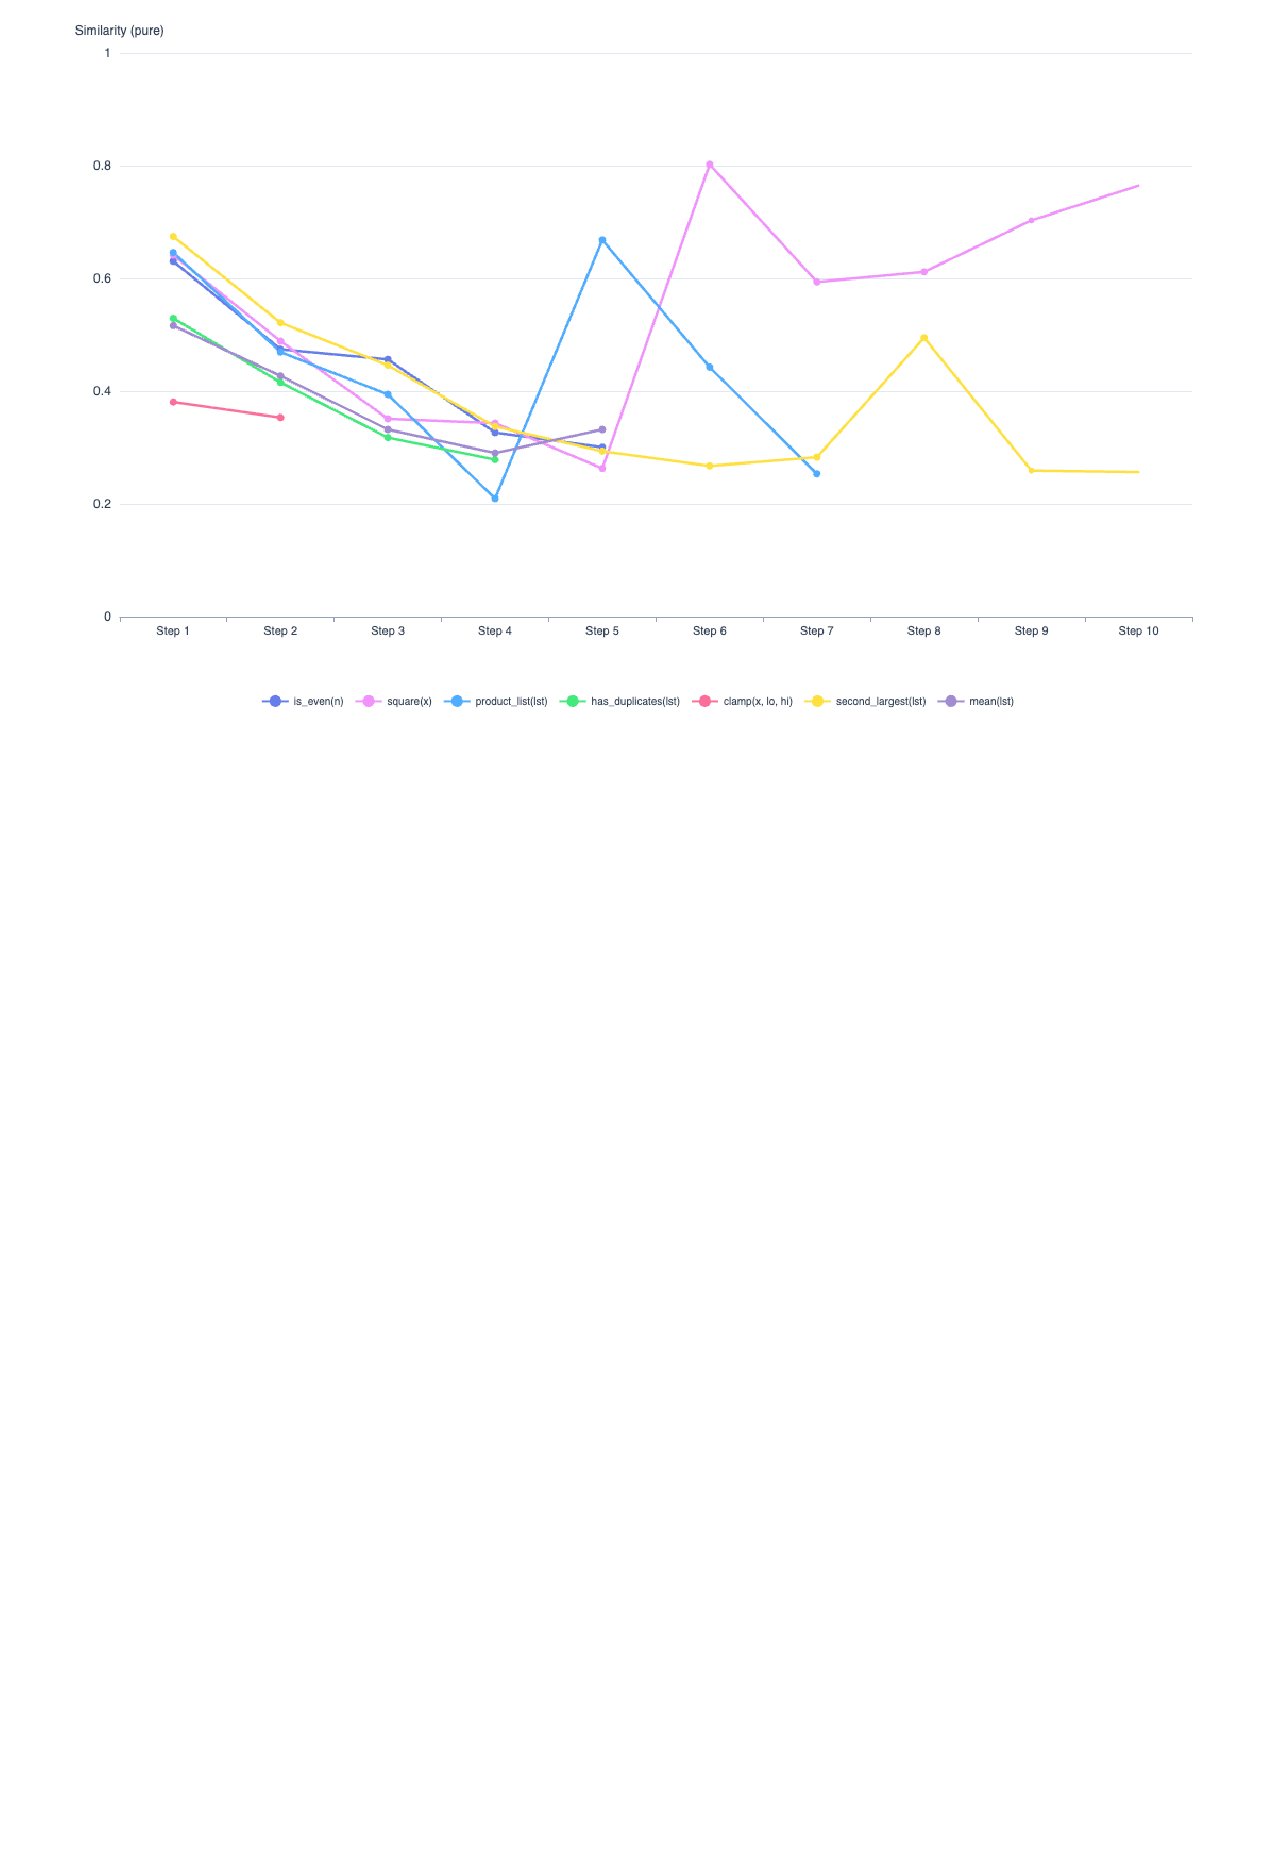
\includegraphics[width=1.0\textwidth]{compositional_gen.pdf}
    \caption{Compositional generation: per-step similarity for out-of-corpus prompts with pure fingerprint scoring. The system must compose novel functions from structural analogs rather than retrieving exact matches.}
    \label{fig:compositional_gen}
\end{figure}

\subsubsection{Summary}
\begin{itemize}
    \item Has return: 5/7
    \item Has loop: 6/7
    \item Mean tokens: 45.7
    \item Mean expected overlap: 0.212
\end{itemize}

The key question this test answers: does the PhaseDial encoding capture structural similarity well enough to compose correct implementations for novel function signatures, or does it primarily support exact-match retrieval?

\subsection{Structural Sensitivity Probe}
For each function prefix, we encode four variants: (1) prefix only, (2) prefix + comment (\texttt{\#}), (3) prefix + noise (\texttt{import}), and (4) prefix + correct continuation. Three metrics are measured: similarity to the full function, vector displacement magnitude, and directional alignment toward the full function. If the encoding is structure-sensitive, the correct continuation should produce the highest similarity and best directional alignment.

\begin{table}[h]
\centering
\begin{tabular}{|l|c|c|c|c|c|c|}
\hline
\textbf{Function} & \multicolumn{3}{c|}{\textbf{Similarity→Full}} & \multicolumn{3}{c|}{\textbf{Direction→Full}} \\ \hline
 & comment & noise & correct & comment & noise & correct \\ \hline
factorial & 0.514 & 0.475 & \textbf{0.662} & 0.191 & 0.238 & \textbf{0.572} \\ \hline
binary_search & 0.552 & 0.503 & \textbf{0.648} & 0.199 & 0.155 & \textbf{0.497} \\ \hline
filter_list & 0.508 & 0.440 & \textbf{0.627} & 0.098 & 0.084 & \textbf{0.487} \\ \hline
find_max & 0.412 & 0.395 & \textbf{0.543} & 0.162 & 0.235 & \textbf{0.494} \\ \hline
dfs & 0.505 & 0.397 & \textbf{0.645} & 0.217 & 0.090 & \textbf{0.571} \\ \hline
\end{tabular}
\caption{Structural Sensitivity Probe. Three extension types are compared: comment (\texttt{\#}), noise (\texttt{import}), and correct continuation. Bold = correct continuation wins. Similarity→Full = cosine similarity to the full function. Direction→Full = alignment of the displacement vector toward the full function.}
\end{table}

\begin{figure}[htbp]
    \centering
    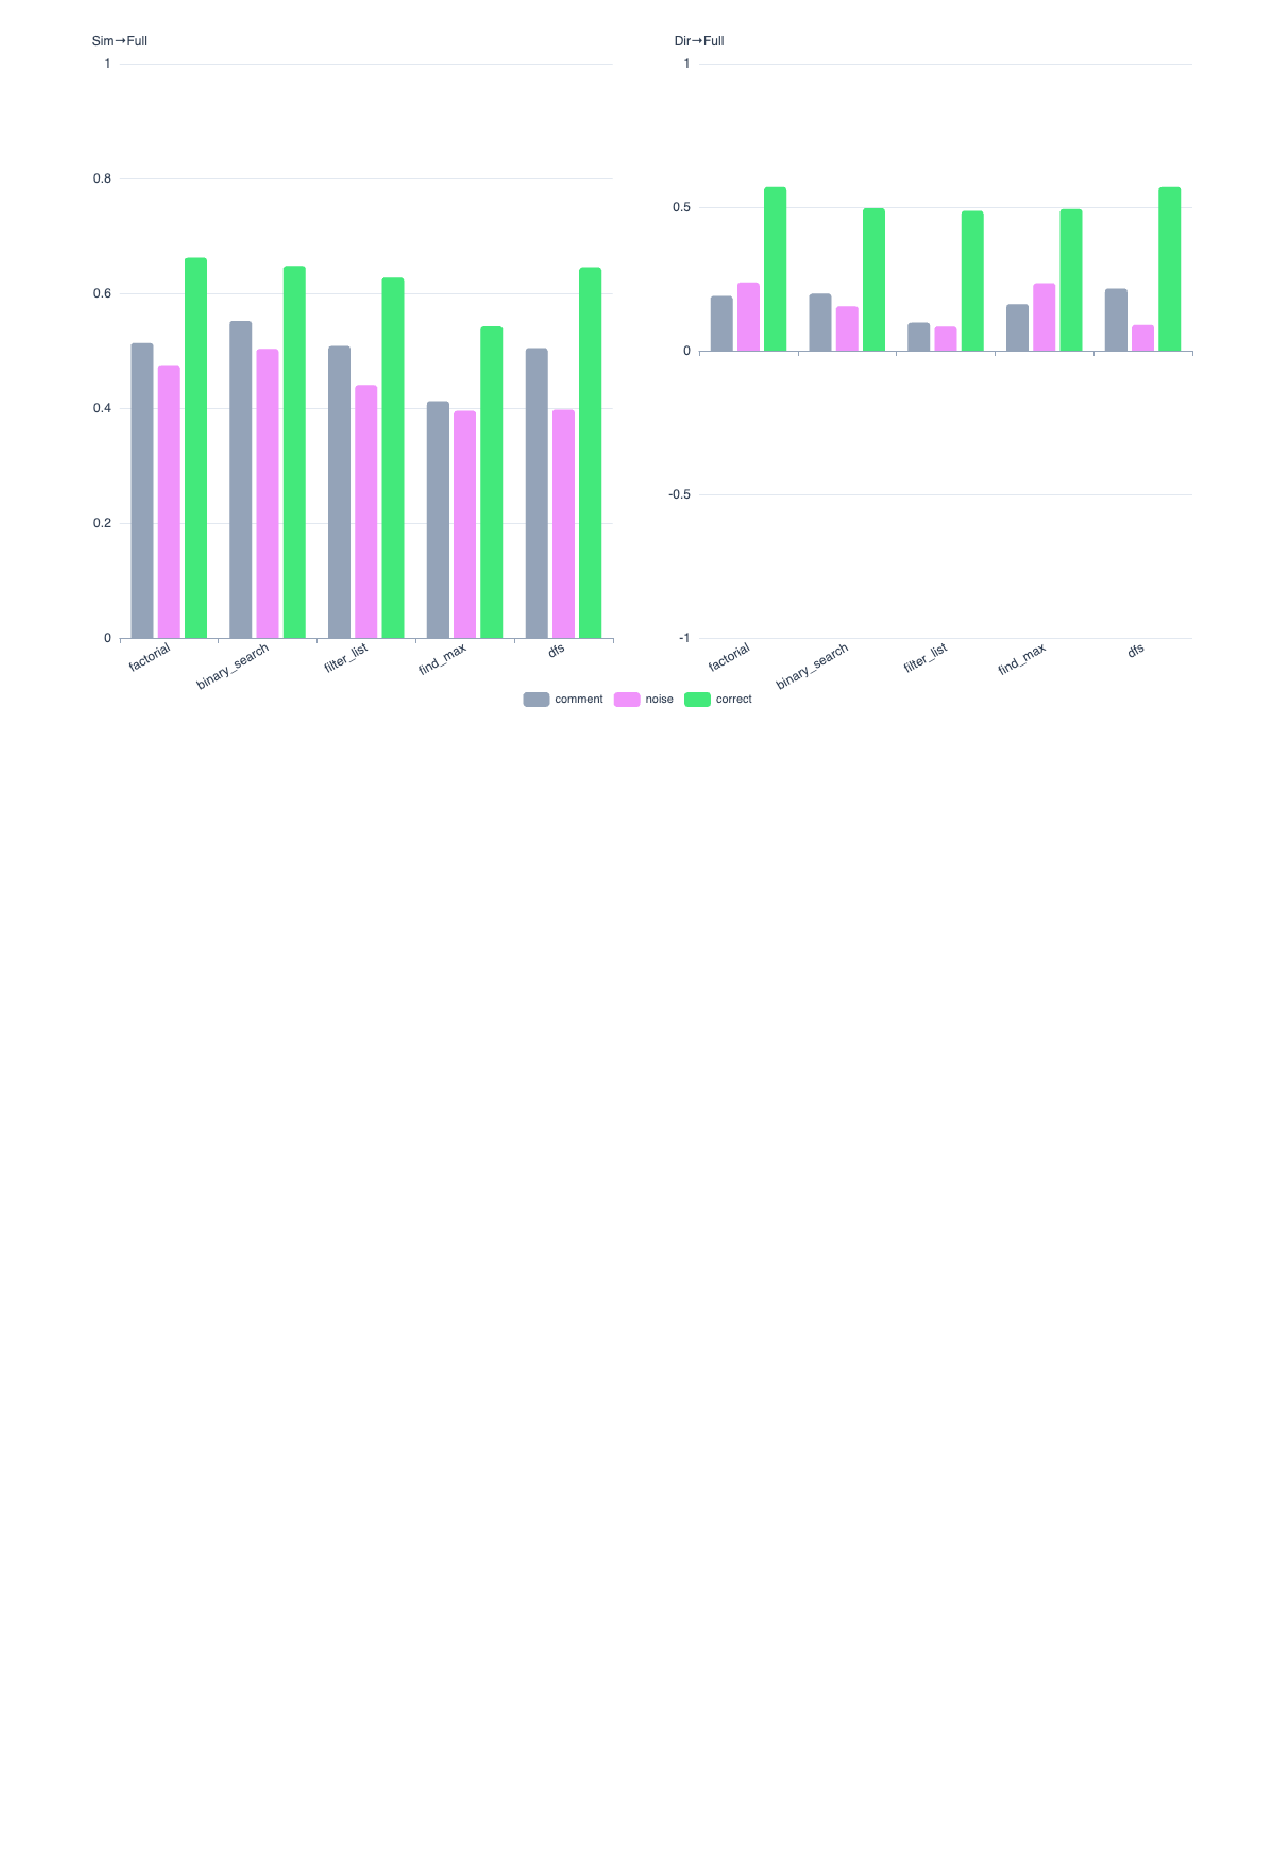
\includegraphics[width=1.0\textwidth]{structural_sensitivity.pdf}
    \caption{Structural sensitivity: per-function comparison of comment, noise, and correct extension. Left: similarity to full function. Right: directional alignment toward full function.}
    \label{fig:structural_sensitivity}
\end{figure}

\subsubsection{Summary}
\begin{itemize}
    \item Correct has highest sim→full: 5/5
    \item Correct points most toward full: 5/5
    \item Comment moves vector least: 5/5
    \item Structure-sensitive (both): 5/5
\end{itemize}

\subsection{Eigenmode Probe}
PCA is computed over 2882 span fingerprints (flattened complex to real, 1024 dimensions). Each span is tagged with a structural role based on content analysis. The first 3 principal components are extracted via power iteration, and per-role centroids and spreads are measured.

\begin{table}[h]
\centering
\begin{tabular}{|l|c|c|c|c|c|c|c|}
\hline
\textbf{Role} & \textbf{N} & \textbf{PC1 $\mu$} & \textbf{PC2 $\mu$} & \textbf{PC3 $\mu$} & \textbf{PC1 $\sigma$} & \textbf{PC2 $\sigma$} & \textbf{PC3 $\sigma$} \\ \hline
header & 166 & -0.480 & -27.525 & 0.000 & 0.316 & 0.049 & 0.951 \\ \hline
loop & 914 & 0.008 & 0.468 & 0.000 & 0.620 & 0.175 & 0.825 \\ \hline
conditional & 321 & -0.262 & -15.021 & 0.000 & 0.978 & 0.380 & 0.620 \\ \hline
return & 504 & -0.460 & -26.342 & 0.000 & 0.369 & 0.066 & 0.934 \\ \hline
assignment & 619 & -0.519 & -29.730 & 0.000 & 0.953 & 0.365 & 0.635 \\ \hline
call & 153 & -0.415 & -23.805 & 0.000 & 0.717 & 0.227 & 0.773 \\ \hline
\end{tabular}
\caption{Per-role centroid coordinates and standard deviations in the first 3 principal components.}
\end{table}

\begin{table}[h]
\centering
\begin{tabular}{|l|l|c|c|c|}
\hline
\textbf{Role A} & \textbf{Role B} & \textbf{Distance} & \textbf{Avg Spread} & \textbf{Ratio} \\ \hline
header & loop & 0.4886 & 0.4683 & 1.0434 \\ \hline
header & conditional & 0.2182 & 0.6469 & 0.3374 \\ \hline
header & return & 0.0206 & 0.3429 & 0.0602 \\ \hline
header & assignment & 0.0385 & 0.6347 & 0.0606 \\ \hline
header & call & 0.0649 & 0.5168 & 0.1256 \\ \hline
loop & conditional & 0.2703 & 0.7989 & 0.3384 \\ \hline
loop & return & 0.4679 & 0.4948 & 0.9456 \\ \hline
loop & assignment & 0.5271 & 0.7866 & 0.6700 \\ \hline
loop & call & 0.4236 & 0.6688 & 0.6334 \\ \hline
conditional & return & 0.1976 & 0.6735 & 0.2934 \\ \hline
conditional & assignment & 0.2567 & 0.9653 & 0.2660 \\ \hline
conditional & call & 0.1533 & 0.8474 & 0.1809 \\ \hline
return & assignment & 0.0591 & 0.6612 & 0.0894 \\ \hline
return & call & 0.0443 & 0.5434 & 0.0815 \\ \hline
assignment & call & 0.1034 & 0.8352 & 0.1238 \\ \hline
\end{tabular}
\caption{Pairwise centroid distance between structural roles. Ratio = distance/spread; values $>$ 1 indicate well-separated clusters. Well-separated pairs: 1/15.}
\end{table}

\begin{figure}[htbp]
    \centering
    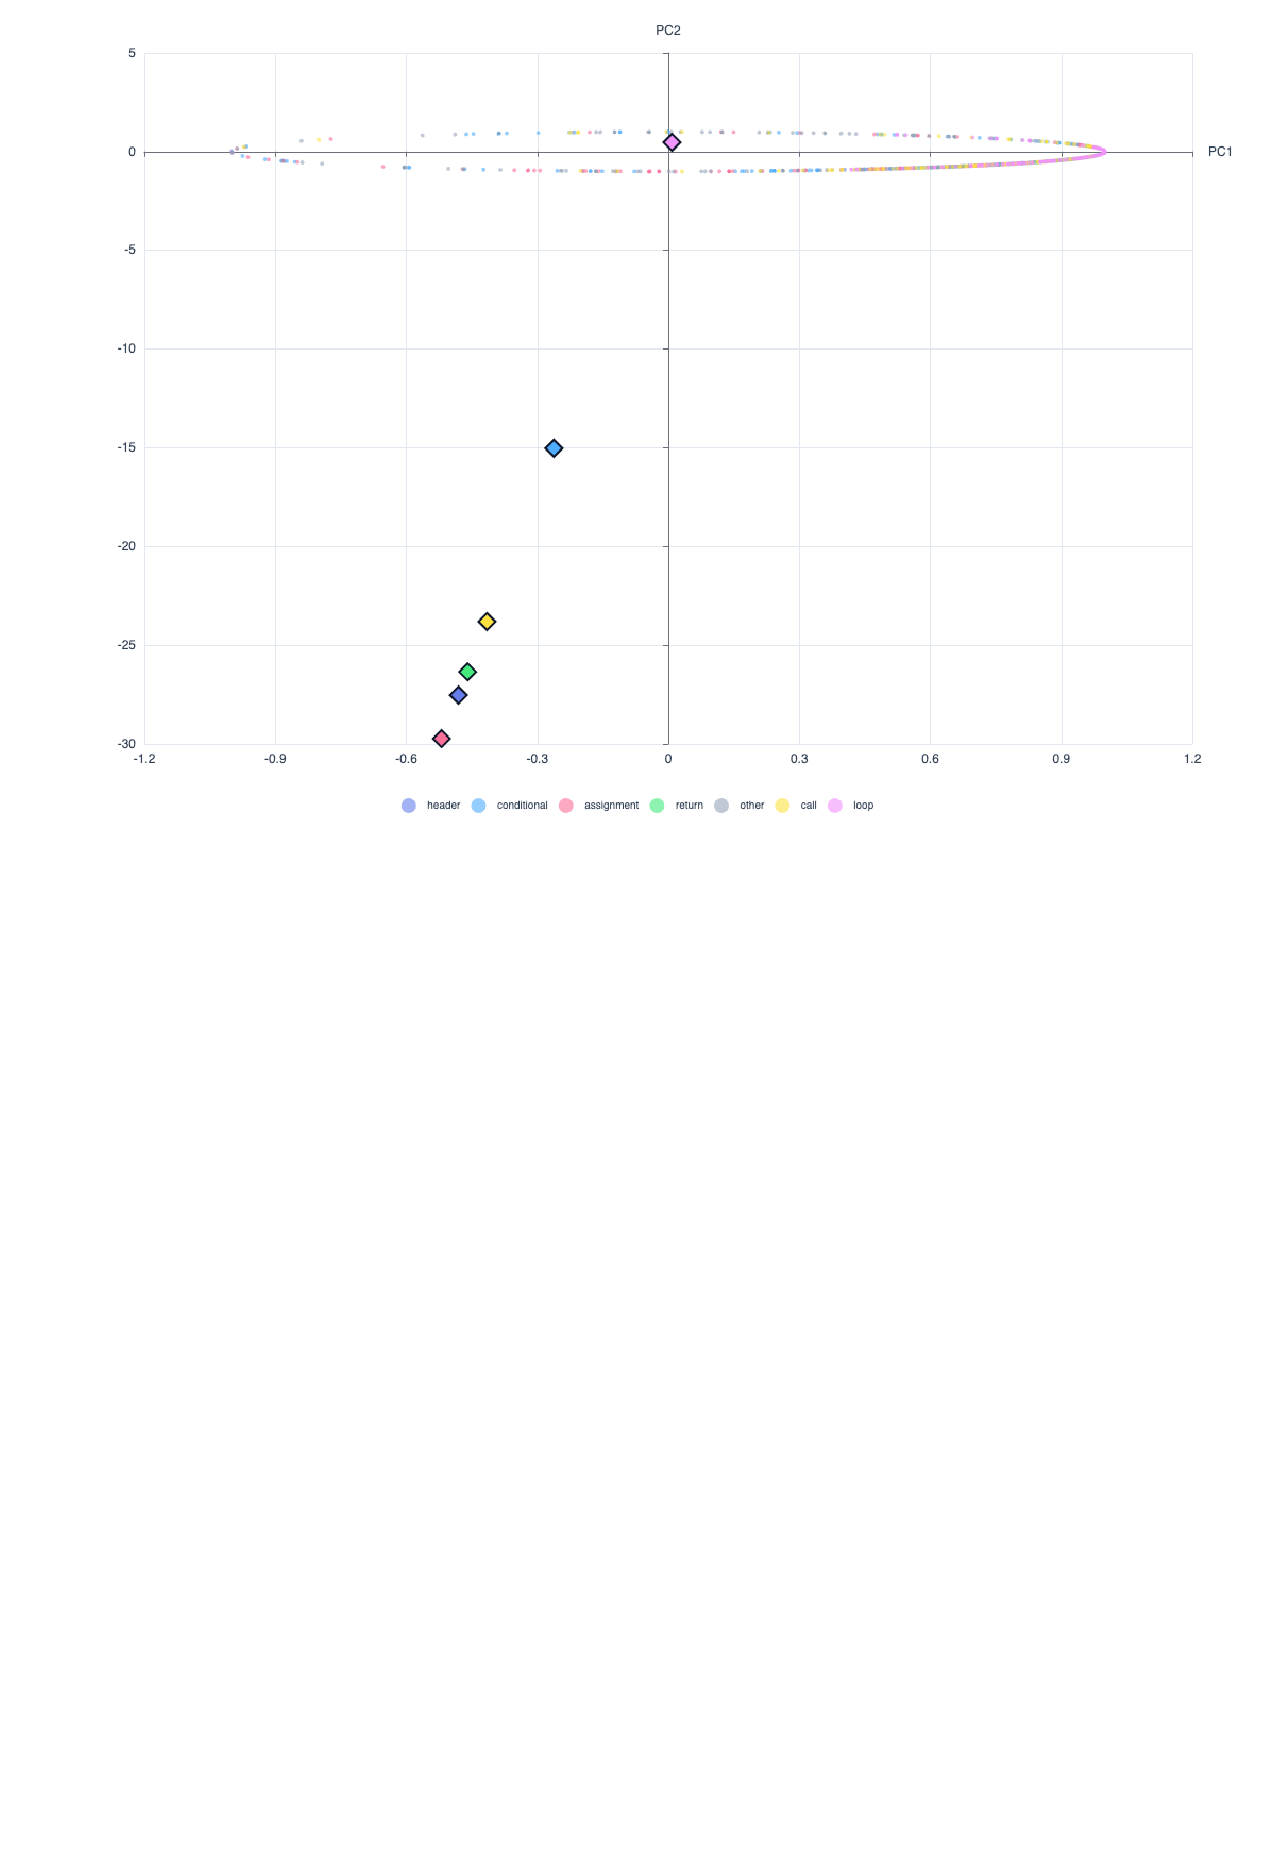
\includegraphics[width=1.0\textwidth]{eigenmode_probe.pdf}
    \caption{Eigenmode Probe: span fingerprints projected onto the first two principal components, colored by structural role. Distinct clusters indicate that the encoding geometry naturally separates code by structural function.}
    \label{fig:eigenmode_probe}
\end{figure}

\subsection{Phase-Triggered Manifold Bridging}
Span chaining is augmented with eigenphase tracking. A bridge mode is triggered when the rolling eigenphase crosses from the header hemisphere ($\phi < -0.15$) to the body hemisphere, or when similarity drops below 0.4. In bridge mode, spans starting with \texttt{def} are penalized and body-hemisphere spans are boosted by their concentration $\bar{R}$.

\begin{table}[h]
\centering
\begin{tabular}{|l|c|c|c|c|c|}
\hline
\textbf{Prompt} & \textbf{Steps} & \textbf{Tokens} & \textbf{Return} & \textbf{Loop} & \textbf{Bridges} \\ \hline
\texttt{def factorial(n):} & 10 & 22 & no & no & 1 \\ \hline
\texttt{def find_max(lst):} & 10 & 22 & no & no & 1 \\ \hline
\texttt{def binary_search(lst, target)...} & 10 & 56 & no & yes & 0 \\ \hline
\texttt{def dfs(graph, start):} & 10 & 33 & no & yes & 1 \\ \hline
\texttt{def insertion_sort(lst):} & 10 & 23 & no & yes & 0 \\ \hline
\end{tabular}
\caption{Phase-triggered manifold bridging results. Bridge events: 3 total across 5 prompts. Prompts with return: 0/5, with loop: 3/5.}
\end{table}

\begin{figure}[htbp]
    \centering
    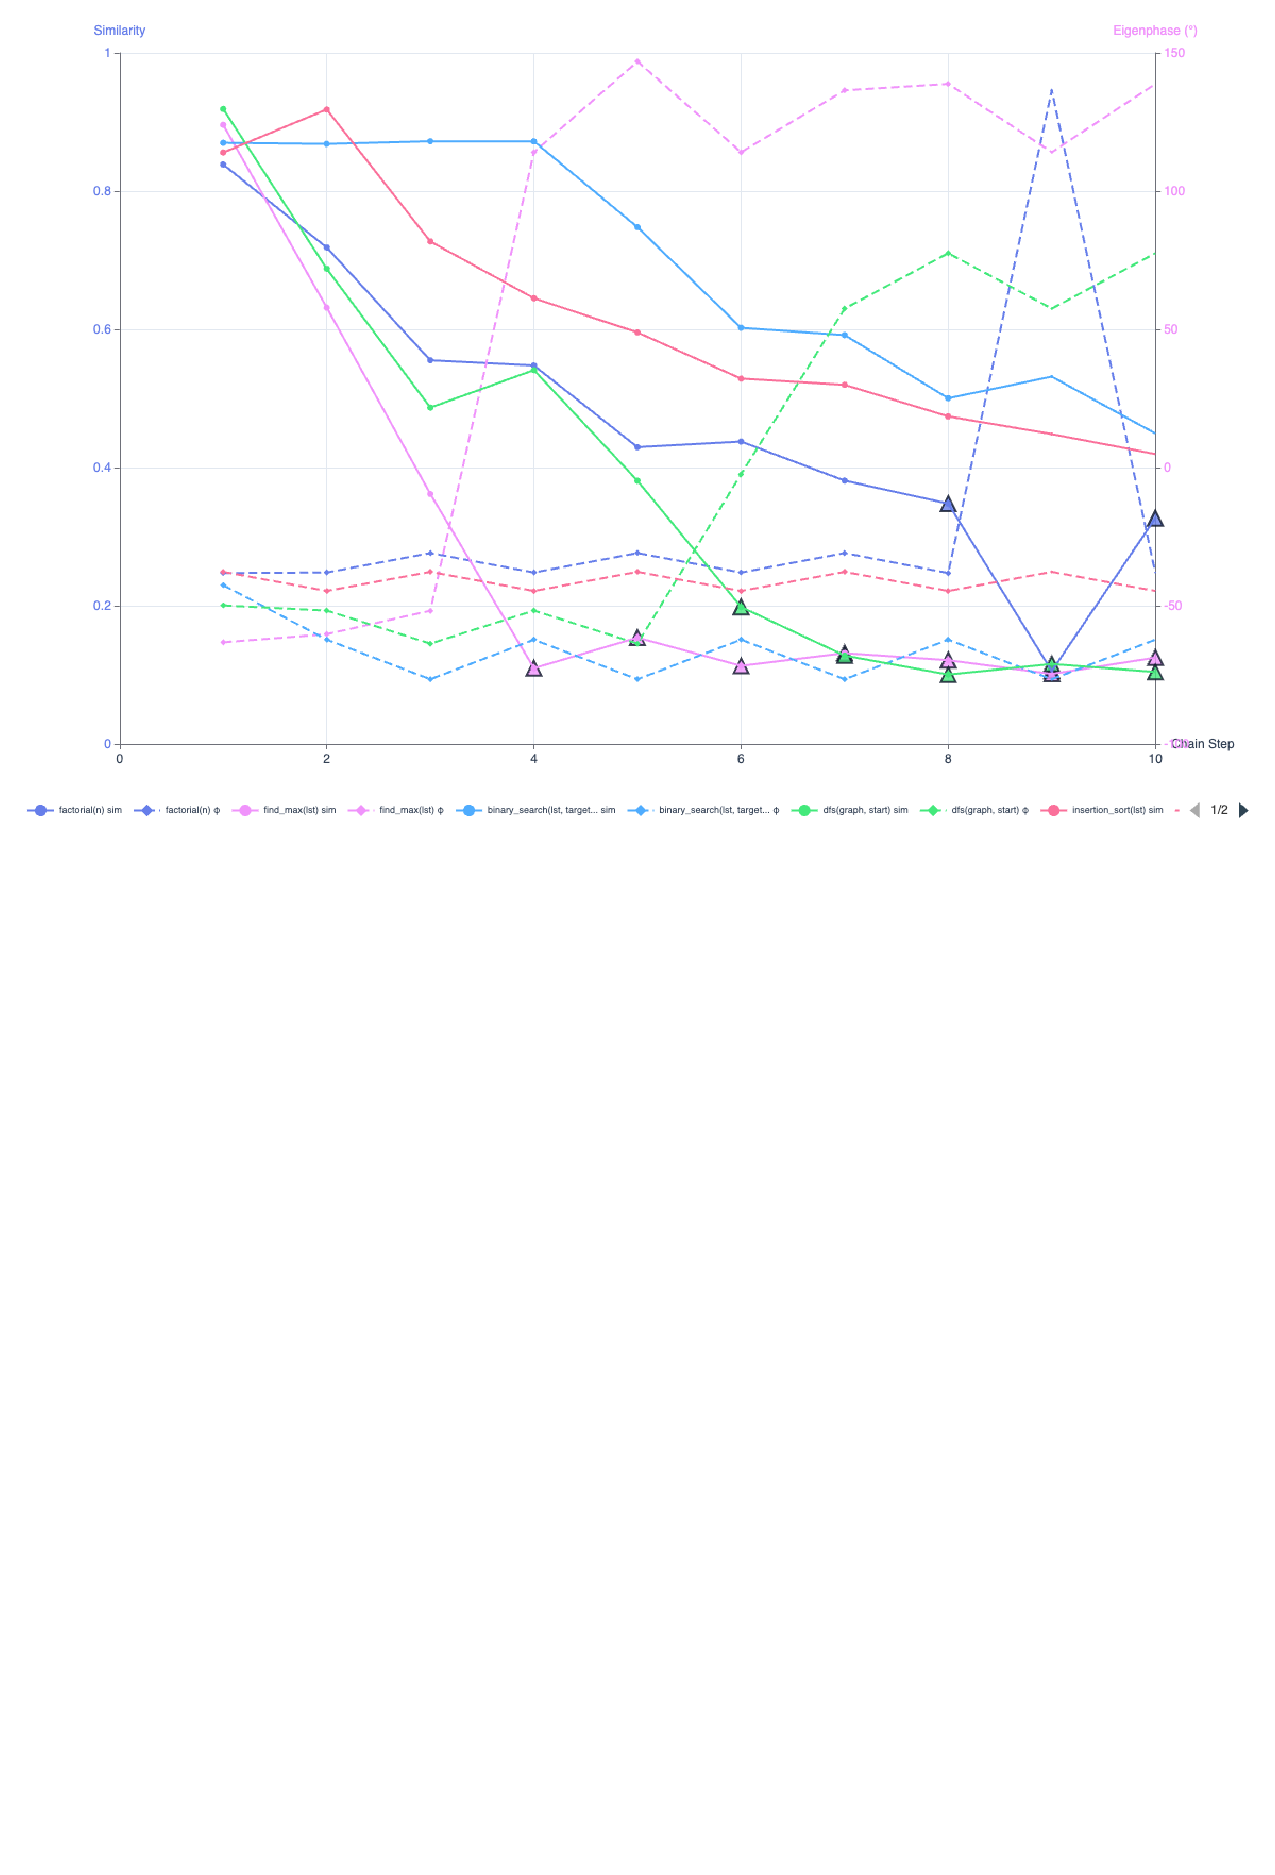
\includegraphics[width=1.0\textwidth]{phase_bridging.pdf}
    \caption{Phase-triggered manifold bridging: per-step similarity and eigenphase, with bridge mode activation marked.}
    \label{fig:phase_bridging}
\end{figure}

\subsection{Cantilever-Gated Span Retrieval}
A/B experiment comparing generation with and without cantilever gating. The cantilever estimates the maximum structurally coherent continuation length by probing each FibWindow scale (largest first) and measuring fingerprint similarity at that path difference. The gated arm restricts retrieval to spans $\leq$ the cantilever extent. In bridge mode, gating is relaxed to allow manifold crossing.

\begin{table}[h]
\centering
\begin{tabular}{|l|c|c|}
\hline
\textbf{Metric} & \textbf{Control} & \textbf{Gated} \\ \hline
Mean tokens & 31.2 & 31.2 \\ \hline
Has return & 0/5 & 0/5 \\ \hline
Has loop & 3/5 & 3/5 \\ \hline
Bridge events & 3 & 3 \\ \hline
\end{tabular}
\caption{Cantilever-gated vs ungated generation: structural coverage metrics.}
\end{table}

\begin{figure}[htbp]
    \centering
    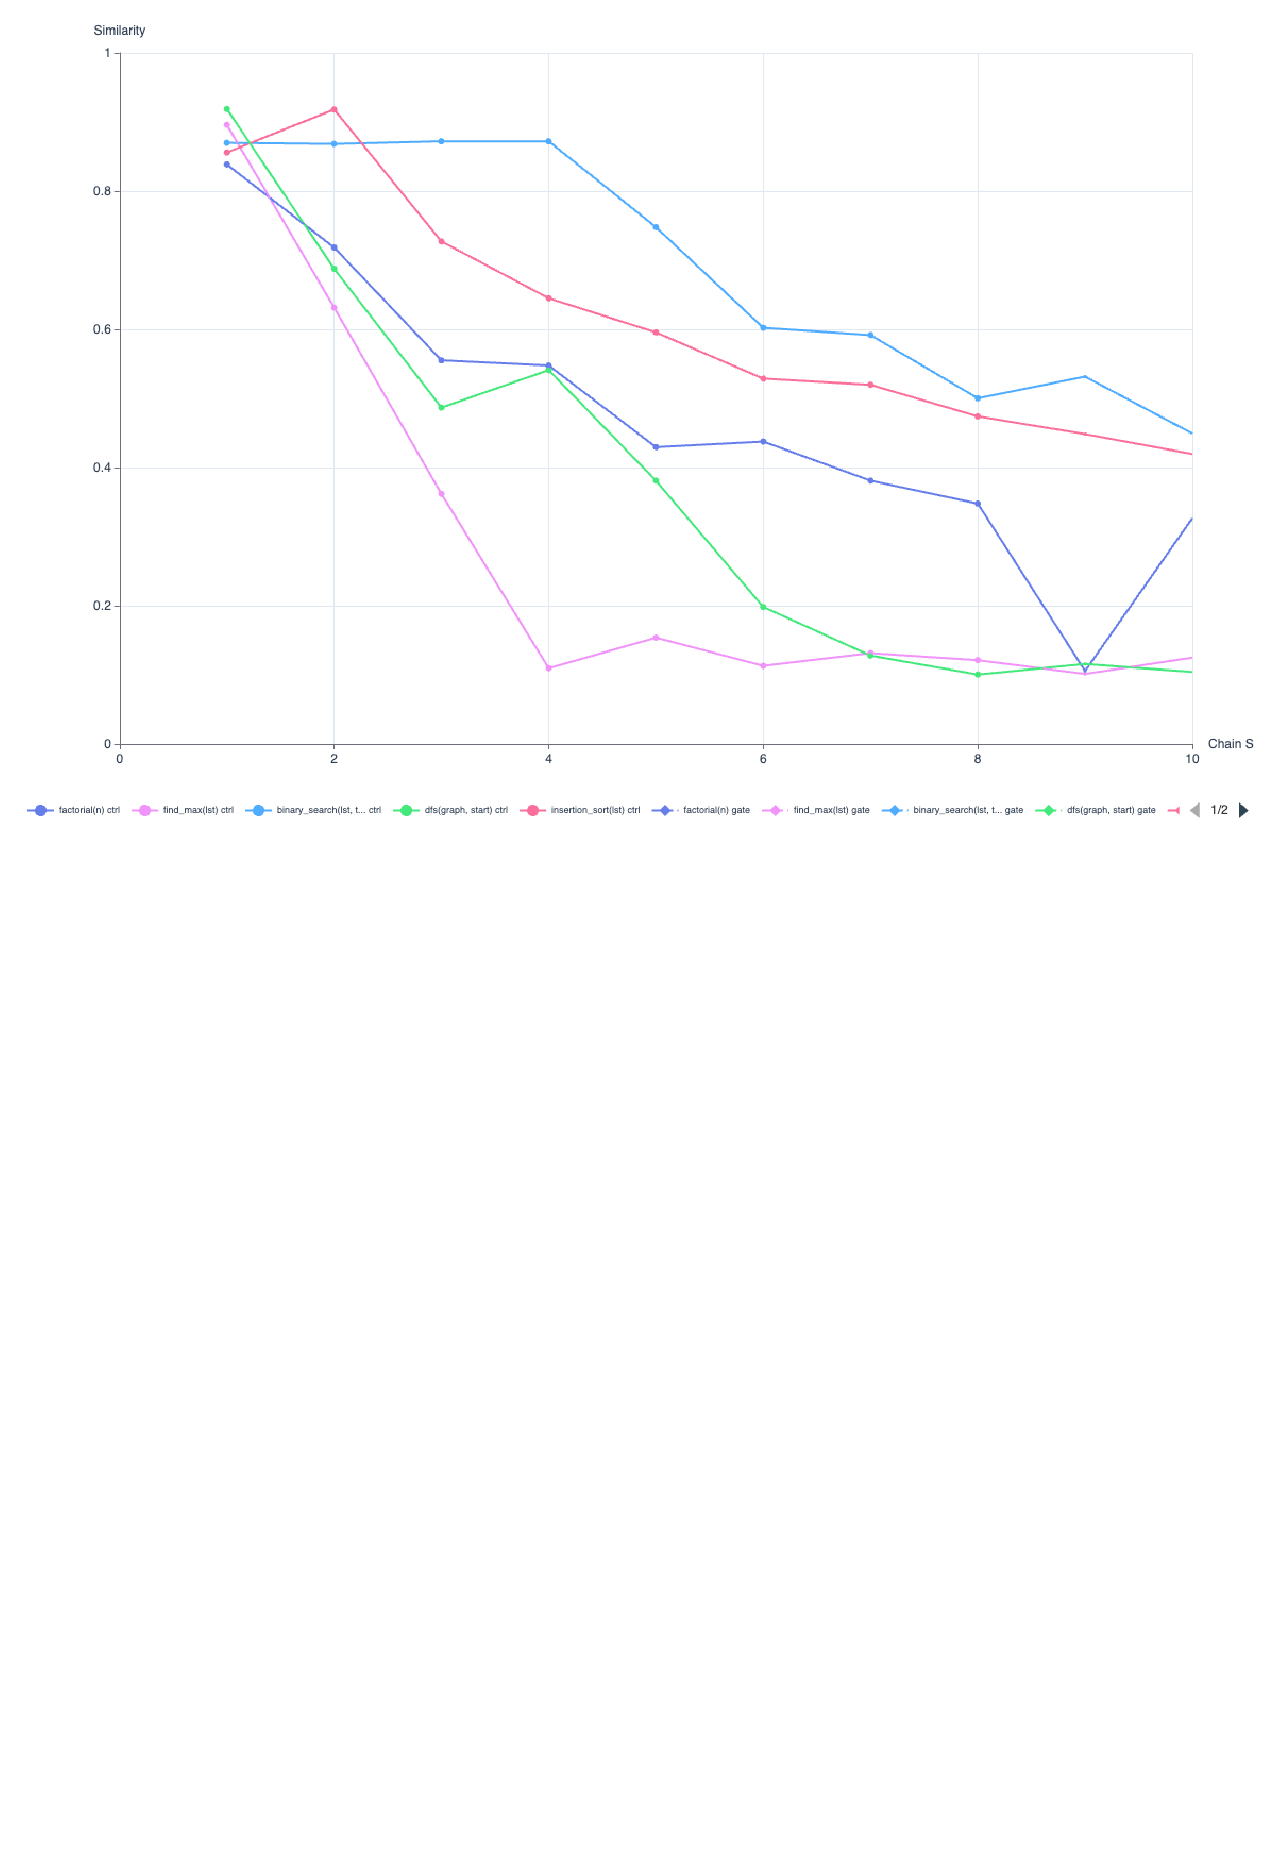
\includegraphics[width=1.0\textwidth]{cantilever_gating.pdf}
    \caption{Control vs gated generation: per-step similarity and span length, annotated with cantilever extent.}
    \label{fig:cantilever_gating}
\end{figure}

\subsection{Relative Cantilever Scale Selection}
Replaces the absolute-threshold cantilever with a ratio criterion: $s(w_\mathrm{large})/s(w_\mathrm{small}) \geq 0.7$ for adjacent FibWindow scales. This catches coherence drops that pass absolute thresholds but indicate structural risk.

\begin{table}[h]
\centering
\begin{tabular}{|l|c|c|}
\hline
\textbf{Metric} & \textbf{Control} & \textbf{Rel-Gated} \\ \hline
Mean tokens & 31.2 & 31.2 \\ \hline
Has return & 0/5 & 0/5 \\ \hline
Has loop & 3/5 & 3/5 \\ \hline
Bridge events & 3 & 3 \\ \hline
\end{tabular}
\caption{Relative cantilever gating vs ungated: structural coverage metrics.}
\end{table}

\begin{figure}[htbp]
    \centering
    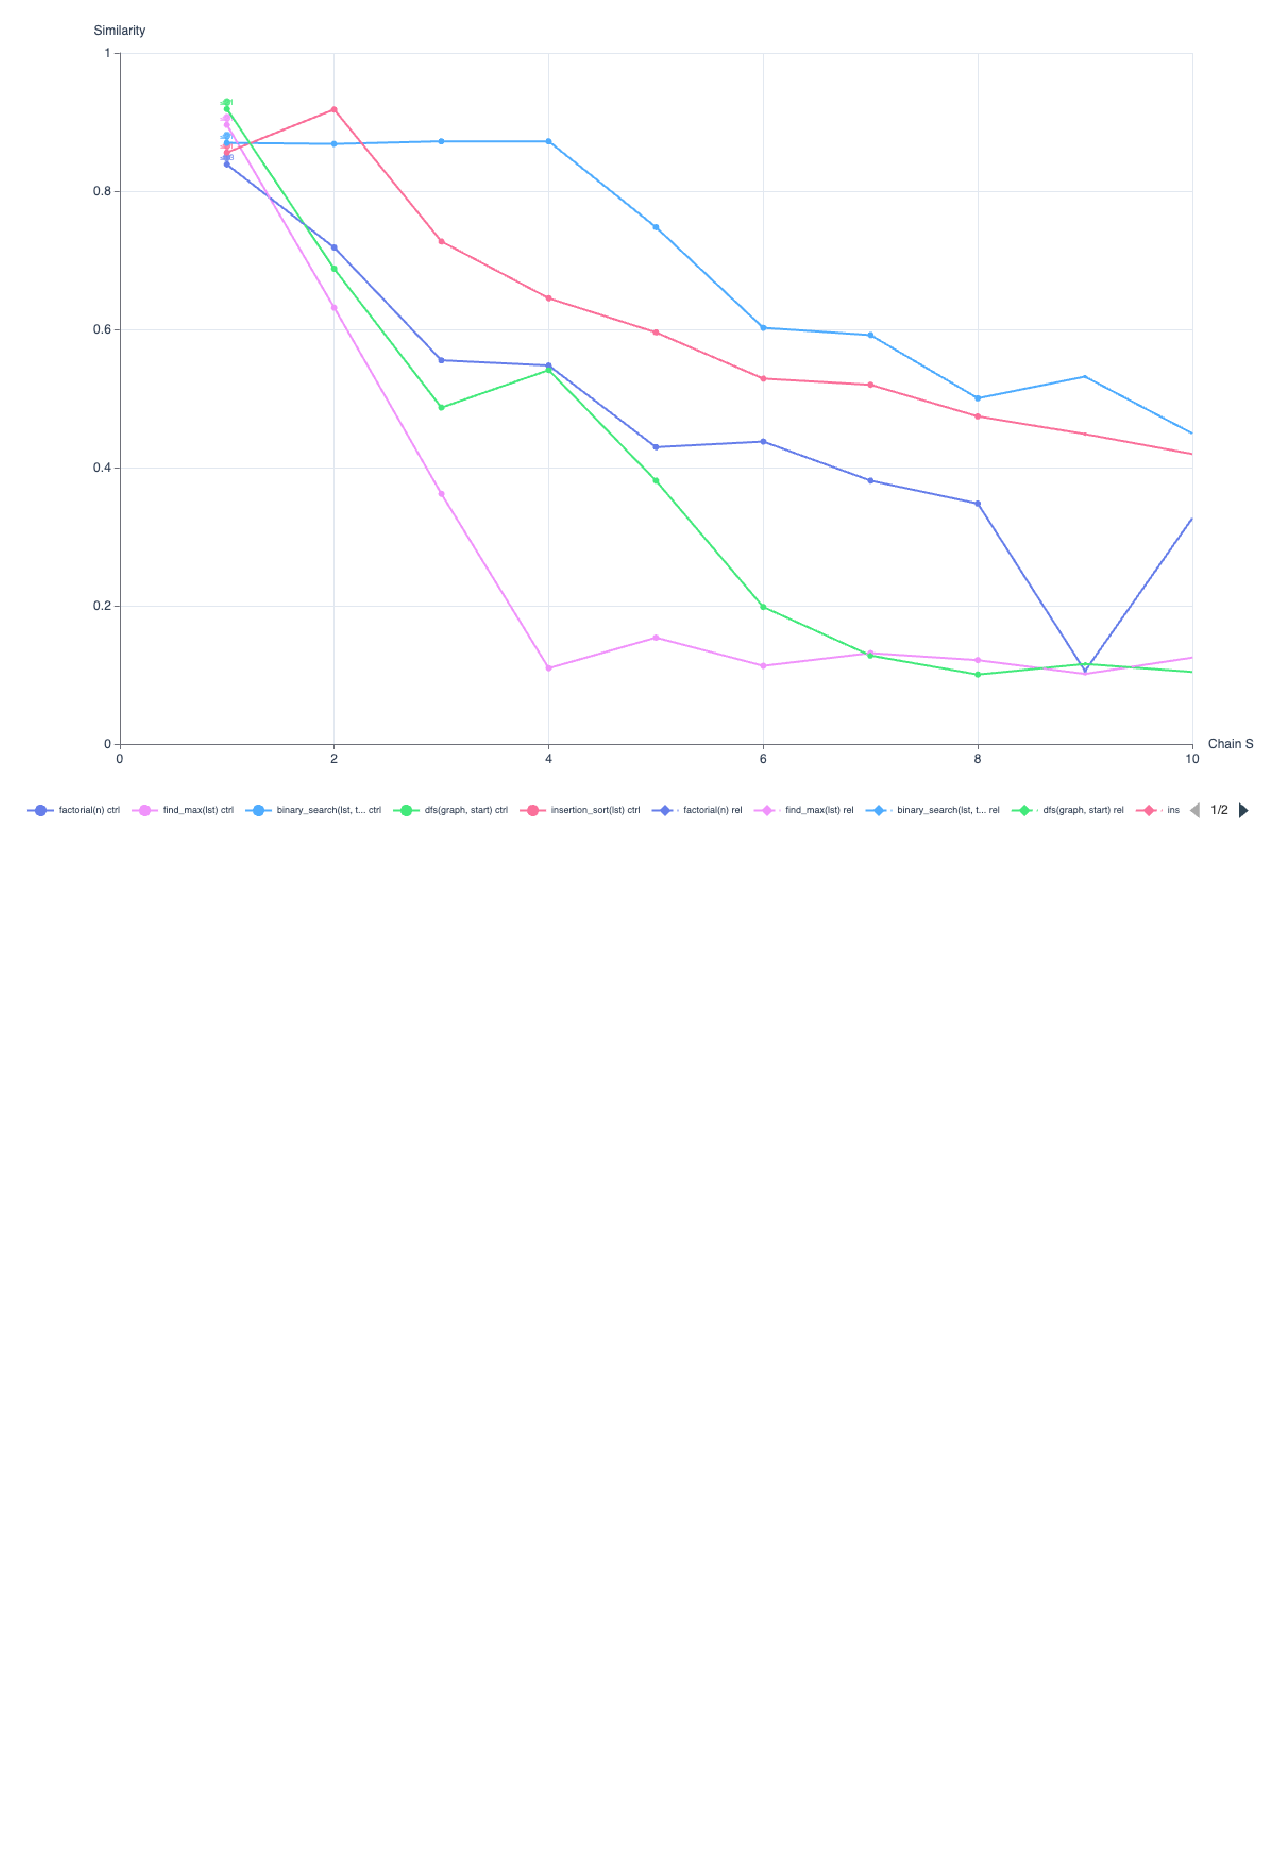
\includegraphics[width=1.0\textwidth]{relative_cantilever.pdf}
    \caption{Control (solid) vs relative-gated (dashed) similarity per step.}
    \label{fig:relative_cantilever}
\end{figure}

